\documentclass[twoside]{book}

% Packages required by doxygen
\usepackage{fixltx2e}
\usepackage{calc}
\usepackage{doxygen}
\usepackage[export]{adjustbox} % also loads graphicx
\usepackage{graphicx}
\usepackage[utf8]{inputenc}
\usepackage{makeidx}
\usepackage{multicol}
\usepackage{multirow}
\PassOptionsToPackage{warn}{textcomp}
\usepackage{textcomp}
\usepackage[nointegrals]{wasysym}
\usepackage[table]{xcolor}

% Font selection
\usepackage[T1]{fontenc}
\usepackage[scaled=.90]{helvet}
\usepackage{courier}
\usepackage{amssymb}
\usepackage{sectsty}
\renewcommand{\familydefault}{\sfdefault}
\allsectionsfont{%
  \fontseries{bc}\selectfont%
  \color{darkgray}%
}
\renewcommand{\DoxyLabelFont}{%
  \fontseries{bc}\selectfont%
  \color{darkgray}%
}
\newcommand{\+}{\discretionary{\mbox{\scriptsize$\hookleftarrow$}}{}{}}

% Page & text layout
\usepackage{geometry}
\geometry{%
  a4paper,%
  top=2.5cm,%
  bottom=2.5cm,%
  left=2.5cm,%
  right=2.5cm%
}
\tolerance=750
\hfuzz=15pt
\hbadness=750
\setlength{\emergencystretch}{15pt}
\setlength{\parindent}{0cm}
\setlength{\parskip}{3ex plus 2ex minus 2ex}
\makeatletter
\renewcommand{\paragraph}{%
  \@startsection{paragraph}{4}{0ex}{-1.0ex}{1.0ex}{%
    \normalfont\normalsize\bfseries\SS@parafont%
  }%
}
\renewcommand{\subparagraph}{%
  \@startsection{subparagraph}{5}{0ex}{-1.0ex}{1.0ex}{%
    \normalfont\normalsize\bfseries\SS@subparafont%
  }%
}
\makeatother

% Headers & footers
\usepackage{fancyhdr}
\pagestyle{fancyplain}
\fancyhead[LE]{\fancyplain{}{\bfseries\thepage}}
\fancyhead[CE]{\fancyplain{}{}}
\fancyhead[RE]{\fancyplain{}{\bfseries\leftmark}}
\fancyhead[LO]{\fancyplain{}{\bfseries\rightmark}}
\fancyhead[CO]{\fancyplain{}{}}
\fancyhead[RO]{\fancyplain{}{\bfseries\thepage}}
\fancyfoot[LE]{\fancyplain{}{}}
\fancyfoot[CE]{\fancyplain{}{}}
\fancyfoot[RE]{\fancyplain{}{\bfseries\scriptsize Generated by Doxygen }}
\fancyfoot[LO]{\fancyplain{}{\bfseries\scriptsize Generated by Doxygen }}
\fancyfoot[CO]{\fancyplain{}{}}
\fancyfoot[RO]{\fancyplain{}{}}
\renewcommand{\footrulewidth}{0.4pt}
\renewcommand{\chaptermark}[1]{%
  \markboth{#1}{}%
}
\renewcommand{\sectionmark}[1]{%
  \markright{\thesection\ #1}%
}

% Indices & bibliography
\usepackage{natbib}
\usepackage[titles]{tocloft}
\setcounter{tocdepth}{3}
\setcounter{secnumdepth}{5}
\makeindex

% Hyperlinks (required, but should be loaded last)
\usepackage{ifpdf}
\ifpdf
  \usepackage[pdftex,pagebackref=true]{hyperref}
\else
  \usepackage[ps2pdf,pagebackref=true]{hyperref}
\fi
\hypersetup{%
  colorlinks=true,%
  linkcolor=blue,%
  citecolor=blue,%
  unicode%
}

% Custom commands
\newcommand{\clearemptydoublepage}{%
  \newpage{\pagestyle{empty}\cleardoublepage}%
}

\usepackage{caption}
\captionsetup{labelsep=space,justification=centering,font={bf},singlelinecheck=off,skip=4pt,position=top}

%===== C O N T E N T S =====

\begin{document}

% Titlepage & ToC
\hypersetup{pageanchor=false,
             bookmarksnumbered=true,
             pdfencoding=unicode
            }
\pagenumbering{alph}
\begin{titlepage}
\vspace*{7cm}
\begin{center}%
{\Large Capstone }\\
\vspace*{1cm}
{\large Generated by Doxygen 1.8.13}\\
\end{center}
\end{titlepage}
\clearemptydoublepage
\pagenumbering{roman}
\tableofcontents
\clearemptydoublepage
\pagenumbering{arabic}
\hypersetup{pageanchor=true}

%--- Begin generated contents ---
\chapter{Namespace Index}
\section{Packages}
Here are the packages with brief descriptions (if available)\+:\begin{DoxyCompactList}
\item\contentsline{section}{\hyperlink{namespace_web_content}{Web\+Content} }{\pageref{namespace_web_content}}{}
\item\contentsline{section}{\hyperlink{namespace_web_content_1_1app}{Web\+Content.\+app} }{\pageref{namespace_web_content_1_1app}}{}
\item\contentsline{section}{\hyperlink{namespace_web_content_1_1classes}{Web\+Content.\+classes} }{\pageref{namespace_web_content_1_1classes}}{}
\end{DoxyCompactList}

\chapter{Hierarchical Index}
\section{Class Hierarchy}
This inheritance list is sorted roughly, but not completely, alphabetically\+:\begin{DoxyCompactList}
\item Model\begin{DoxyCompactList}
\item \contentsline{section}{Web\+Content.\+classes.\+allocation\+\_\+table}{\pageref{class_web_content_1_1classes_1_1allocation__table}}{}
\item \contentsline{section}{Web\+Content.\+classes.\+contacts}{\pageref{class_web_content_1_1classes_1_1contacts}}{}
\item \contentsline{section}{Web\+Content.\+classes.\+daily\+\_\+task}{\pageref{class_web_content_1_1classes_1_1daily__task}}{}
\item \contentsline{section}{Web\+Content.\+classes.\+items}{\pageref{class_web_content_1_1classes_1_1items}}{}
\item \contentsline{section}{Web\+Content.\+classes.\+job\+Gear}{\pageref{class_web_content_1_1classes_1_1job_gear}}{}
\item \contentsline{section}{Web\+Content.\+classes.\+Shows}{\pageref{class_web_content_1_1classes_1_1_shows}}{}
\item \contentsline{section}{Web\+Content.\+classes.\+types}{\pageref{class_web_content_1_1classes_1_1types}}{}
\item \contentsline{section}{Web\+Content.\+classes.\+users}{\pageref{class_web_content_1_1classes_1_1users}}{}
\item \contentsline{section}{Web\+Content.\+classes.\+venues}{\pageref{class_web_content_1_1classes_1_1venues}}{}
\end{DoxyCompactList}
\end{DoxyCompactList}

\chapter{Class Index}
\section{Class List}
Here are the classes, structs, unions and interfaces with brief descriptions\+:\begin{DoxyCompactList}
\item\contentsline{section}{\hyperlink{class_web_content_1_1classes_1_1contacts}{Web\+Content.\+classes.\+contacts} }{\pageref{class_web_content_1_1classes_1_1contacts}}{}
\item\contentsline{section}{\hyperlink{class_web_content_1_1classes_1_1items}{Web\+Content.\+classes.\+items} }{\pageref{class_web_content_1_1classes_1_1items}}{}
\item\contentsline{section}{\hyperlink{class_web_content_1_1classes_1_1job_gear}{Web\+Content.\+classes.\+job\+Gear} }{\pageref{class_web_content_1_1classes_1_1job_gear}}{}
\item\contentsline{section}{\hyperlink{class_web_content_1_1classes_1_1_shows}{Web\+Content.\+classes.\+Shows} }{\pageref{class_web_content_1_1classes_1_1_shows}}{}
\item\contentsline{section}{\hyperlink{class_web_content_1_1classes_1_1types}{Web\+Content.\+classes.\+types} }{\pageref{class_web_content_1_1classes_1_1types}}{}
\item\contentsline{section}{\hyperlink{class_web_content_1_1classes_1_1users}{Web\+Content.\+classes.\+users} }{\pageref{class_web_content_1_1classes_1_1users}}{}
\item\contentsline{section}{\hyperlink{class_web_content_1_1classes_1_1venues}{Web\+Content.\+classes.\+venues} }{\pageref{class_web_content_1_1classes_1_1venues}}{}
\end{DoxyCompactList}

\chapter{File Index}
\section{File List}
Here is a list of all files with brief descriptions\+:\begin{DoxyCompactList}
\item\contentsline{section}{\hyperlink{____init_____8py}{\+\_\+\+\_\+init\+\_\+\+\_\+.\+py} }{\pageref{____init_____8py}}{}
\item\contentsline{section}{\hyperlink{app_8py}{app.\+py} }{\pageref{app_8py}}{}
\item\contentsline{section}{\hyperlink{classes_8py}{classes.\+py} }{\pageref{classes_8py}}{}
\end{DoxyCompactList}

\chapter{Namespace Documentation}
\hypertarget{namespace_web_content}{}\section{Web\+Content Namespace Reference}
\label{namespace_web_content}\index{Web\+Content@{Web\+Content}}
\subsection*{Namespaces}
\begin{DoxyCompactItemize}
\item 
 \hyperlink{namespace_web_content_1_1app}{app}
\item 
 \hyperlink{namespace_web_content_1_1classes}{classes}
\end{DoxyCompactItemize}

\hypertarget{namespace_web_content_1_1app}{}\section{Web\+Content.\+app Namespace Reference}
\label{namespace_web_content_1_1app}\index{Web\+Content.\+app@{Web\+Content.\+app}}
\subsection*{Functions}
\begin{DoxyCompactItemize}
\item 
def \hyperlink{namespace_web_content_1_1app_ab0090e2c92ec892cf11fed49d580737a}{home} ()
\item 
def \hyperlink{namespace_web_content_1_1app_ac220a4f6d552ae239a9fe5a933eb4c0d}{welcome} ()
\item 
def \hyperlink{namespace_web_content_1_1app_a1e55cf68c2c2c883c82749a8725e068c}{login} ()
\item 
def \hyperlink{namespace_web_content_1_1app_aeb0d3df489a674be05033bd0ba98e7a6}{database} ()
\item 
def \hyperlink{namespace_web_content_1_1app_a01e890f5f74756a5e0db012e87a3bb32}{add} ()
\item 
def \hyperlink{namespace_web_content_1_1app_a2f6071690c83608f94abb72589ab7527}{update} (id\+Items)
\item 
def \hyperlink{namespace_web_content_1_1app_a280b9c530dfd4125df19a186218bb132}{delete} (id\+Items)
\item 
def \hyperlink{namespace_web_content_1_1app_a368b9d1da5b4c987484797ecce9aabc9}{calendar} ()
\item 
def \hyperlink{namespace_web_content_1_1app_a6d7ee2ff030bada6042b07189d92a01c}{search} ()
\item 
def \hyperlink{namespace_web_content_1_1app_afe68584aa29f9b47108d88d14650c05f}{account} ()
\end{DoxyCompactItemize}
\subsection*{Variables}
\begin{DoxyCompactItemize}
\item 
\hyperlink{namespace_web_content_1_1app_a52716e6e08bae668f90c903a1f4e2f10}{app} = Flask(\+\_\+\+\_\+name\+\_\+\+\_\+)
\item 
\hyperlink{namespace_web_content_1_1app_a317646b91bdcf24c176d3bfc065083f3}{db} = S\+Q\+L\+Alchemy(\hyperlink{namespace_web_content_1_1app_a52716e6e08bae668f90c903a1f4e2f10}{app})
\item 
\hyperlink{namespace_web_content_1_1app_a6092358451315e755637b56d42326052}{secret\+\_\+key}
\item 
\hyperlink{namespace_web_content_1_1app_ac91170bea34c6458f4262824618a18a2}{debug}
\end{DoxyCompactItemize}


\subsection{Function Documentation}
\mbox{\Hypertarget{namespace_web_content_1_1app_afe68584aa29f9b47108d88d14650c05f}\label{namespace_web_content_1_1app_afe68584aa29f9b47108d88d14650c05f}} 
\index{Web\+Content\+::app@{Web\+Content\+::app}!account@{account}}
\index{account@{account}!Web\+Content\+::app@{Web\+Content\+::app}}
\subsubsection{\texorpdfstring{account()}{account()}}
{\footnotesize\ttfamily def Web\+Content.\+app.\+account (\begin{DoxyParamCaption}{ }\end{DoxyParamCaption})}

\begin{DoxyVerb}The function is used to render the page used
on the account rep side.
This includes the ability to create, edit, and delete shows.
\end{DoxyVerb}
 \mbox{\Hypertarget{namespace_web_content_1_1app_a01e890f5f74756a5e0db012e87a3bb32}\label{namespace_web_content_1_1app_a01e890f5f74756a5e0db012e87a3bb32}} 
\index{Web\+Content\+::app@{Web\+Content\+::app}!add@{add}}
\index{add@{add}!Web\+Content\+::app@{Web\+Content\+::app}}
\subsubsection{\texorpdfstring{add()}{add()}}
{\footnotesize\ttfamily def Web\+Content.\+app.\+add (\begin{DoxyParamCaption}{ }\end{DoxyParamCaption})}

\begin{DoxyVerb}This function will be used to add new items into inventory
This ability will only be given to select personal.
\end{DoxyVerb}
 \mbox{\Hypertarget{namespace_web_content_1_1app_a368b9d1da5b4c987484797ecce9aabc9}\label{namespace_web_content_1_1app_a368b9d1da5b4c987484797ecce9aabc9}} 
\index{Web\+Content\+::app@{Web\+Content\+::app}!calendar@{calendar}}
\index{calendar@{calendar}!Web\+Content\+::app@{Web\+Content\+::app}}
\subsubsection{\texorpdfstring{calendar()}{calendar()}}
{\footnotesize\ttfamily def Web\+Content.\+app.\+calendar (\begin{DoxyParamCaption}{ }\end{DoxyParamCaption})}

\begin{DoxyVerb}Rednders a calender.
The calender will make it easier to visualize
gear and their locations to aviod confilicts.
\end{DoxyVerb}
 \mbox{\Hypertarget{namespace_web_content_1_1app_aeb0d3df489a674be05033bd0ba98e7a6}\label{namespace_web_content_1_1app_aeb0d3df489a674be05033bd0ba98e7a6}} 
\index{Web\+Content\+::app@{Web\+Content\+::app}!database@{database}}
\index{database@{database}!Web\+Content\+::app@{Web\+Content\+::app}}
\subsubsection{\texorpdfstring{database()}{database()}}
{\footnotesize\ttfamily def Web\+Content.\+app.\+database (\begin{DoxyParamCaption}{ }\end{DoxyParamCaption})}

\begin{DoxyVerb}Gives access to the inventory
with the ability to add, edit, and delete
inventory only select users will have that privlege.
\end{DoxyVerb}
 \mbox{\Hypertarget{namespace_web_content_1_1app_a280b9c530dfd4125df19a186218bb132}\label{namespace_web_content_1_1app_a280b9c530dfd4125df19a186218bb132}} 
\index{Web\+Content\+::app@{Web\+Content\+::app}!delete@{delete}}
\index{delete@{delete}!Web\+Content\+::app@{Web\+Content\+::app}}
\subsubsection{\texorpdfstring{delete()}{delete()}}
{\footnotesize\ttfamily def Web\+Content.\+app.\+delete (\begin{DoxyParamCaption}\item[{}]{id\+Items }\end{DoxyParamCaption})}

\begin{DoxyVerb}This function give the user the
ability to delete items from inventory.
\end{DoxyVerb}
 \mbox{\Hypertarget{namespace_web_content_1_1app_ab0090e2c92ec892cf11fed49d580737a}\label{namespace_web_content_1_1app_ab0090e2c92ec892cf11fed49d580737a}} 
\index{Web\+Content\+::app@{Web\+Content\+::app}!home@{home}}
\index{home@{home}!Web\+Content\+::app@{Web\+Content\+::app}}
\subsubsection{\texorpdfstring{home()}{home()}}
{\footnotesize\ttfamily def Web\+Content.\+app.\+home (\begin{DoxyParamCaption}{ }\end{DoxyParamCaption})}

\begin{DoxyVerb}Redircts to the login page.
\end{DoxyVerb}
 \mbox{\Hypertarget{namespace_web_content_1_1app_a1e55cf68c2c2c883c82749a8725e068c}\label{namespace_web_content_1_1app_a1e55cf68c2c2c883c82749a8725e068c}} 
\index{Web\+Content\+::app@{Web\+Content\+::app}!login@{login}}
\index{login@{login}!Web\+Content\+::app@{Web\+Content\+::app}}
\subsubsection{\texorpdfstring{login()}{login()}}
{\footnotesize\ttfamily def Web\+Content.\+app.\+login (\begin{DoxyParamCaption}{ }\end{DoxyParamCaption})}

\begin{DoxyVerb}The login page
users will provide a username and password if correct
will direct them to the welcome/main page.
\end{DoxyVerb}
 \mbox{\Hypertarget{namespace_web_content_1_1app_a6d7ee2ff030bada6042b07189d92a01c}\label{namespace_web_content_1_1app_a6d7ee2ff030bada6042b07189d92a01c}} 
\index{Web\+Content\+::app@{Web\+Content\+::app}!search@{search}}
\index{search@{search}!Web\+Content\+::app@{Web\+Content\+::app}}
\subsubsection{\texorpdfstring{search()}{search()}}
{\footnotesize\ttfamily def Web\+Content.\+app.\+search (\begin{DoxyParamCaption}{ }\end{DoxyParamCaption})}

\begin{DoxyVerb}This function lets the user search
through the database.
\end{DoxyVerb}
 \mbox{\Hypertarget{namespace_web_content_1_1app_a2f6071690c83608f94abb72589ab7527}\label{namespace_web_content_1_1app_a2f6071690c83608f94abb72589ab7527}} 
\index{Web\+Content\+::app@{Web\+Content\+::app}!update@{update}}
\index{update@{update}!Web\+Content\+::app@{Web\+Content\+::app}}
\subsubsection{\texorpdfstring{update()}{update()}}
{\footnotesize\ttfamily def Web\+Content.\+app.\+update (\begin{DoxyParamCaption}\item[{}]{id\+Items }\end{DoxyParamCaption})}

\begin{DoxyVerb}Lets the user edit items already in inventory.
Only select users will be able to modify inventory.
\end{DoxyVerb}
 \mbox{\Hypertarget{namespace_web_content_1_1app_ac220a4f6d552ae239a9fe5a933eb4c0d}\label{namespace_web_content_1_1app_ac220a4f6d552ae239a9fe5a933eb4c0d}} 
\index{Web\+Content\+::app@{Web\+Content\+::app}!welcome@{welcome}}
\index{welcome@{welcome}!Web\+Content\+::app@{Web\+Content\+::app}}
\subsubsection{\texorpdfstring{welcome()}{welcome()}}
{\footnotesize\ttfamily def Web\+Content.\+app.\+welcome (\begin{DoxyParamCaption}{ }\end{DoxyParamCaption})}

\begin{DoxyVerb}This will the main page for users
that work. They will be able to check status on inventory
and assign them to shows.
\end{DoxyVerb}
 

\subsection{Variable Documentation}
\mbox{\Hypertarget{namespace_web_content_1_1app_a52716e6e08bae668f90c903a1f4e2f10}\label{namespace_web_content_1_1app_a52716e6e08bae668f90c903a1f4e2f10}} 
\index{Web\+Content\+::app@{Web\+Content\+::app}!app@{app}}
\index{app@{app}!Web\+Content\+::app@{Web\+Content\+::app}}
\subsubsection{\texorpdfstring{app}{app}}
{\footnotesize\ttfamily Web\+Content.\+app.\+app = Flask(\+\_\+\+\_\+name\+\_\+\+\_\+)}

\mbox{\Hypertarget{namespace_web_content_1_1app_a317646b91bdcf24c176d3bfc065083f3}\label{namespace_web_content_1_1app_a317646b91bdcf24c176d3bfc065083f3}} 
\index{Web\+Content\+::app@{Web\+Content\+::app}!db@{db}}
\index{db@{db}!Web\+Content\+::app@{Web\+Content\+::app}}
\subsubsection{\texorpdfstring{db}{db}}
{\footnotesize\ttfamily Web\+Content.\+app.\+db = S\+Q\+L\+Alchemy(\hyperlink{namespace_web_content_1_1app_a52716e6e08bae668f90c903a1f4e2f10}{app})}

\mbox{\Hypertarget{namespace_web_content_1_1app_ac91170bea34c6458f4262824618a18a2}\label{namespace_web_content_1_1app_ac91170bea34c6458f4262824618a18a2}} 
\index{Web\+Content\+::app@{Web\+Content\+::app}!debug@{debug}}
\index{debug@{debug}!Web\+Content\+::app@{Web\+Content\+::app}}
\subsubsection{\texorpdfstring{debug}{debug}}
{\footnotesize\ttfamily Web\+Content.\+app.\+debug}

\mbox{\Hypertarget{namespace_web_content_1_1app_a6092358451315e755637b56d42326052}\label{namespace_web_content_1_1app_a6092358451315e755637b56d42326052}} 
\index{Web\+Content\+::app@{Web\+Content\+::app}!secret\+\_\+key@{secret\+\_\+key}}
\index{secret\+\_\+key@{secret\+\_\+key}!Web\+Content\+::app@{Web\+Content\+::app}}
\subsubsection{\texorpdfstring{secret\+\_\+key}{secret\_key}}
{\footnotesize\ttfamily Web\+Content.\+app.\+secret\+\_\+key}


\hypertarget{namespace_web_content_1_1classes}{}\section{Web\+Content.\+classes Namespace Reference}
\label{namespace_web_content_1_1classes}\index{Web\+Content.\+classes@{Web\+Content.\+classes}}
\subsection*{Classes}
\begin{DoxyCompactItemize}
\item 
class \hyperlink{class_web_content_1_1classes_1_1contacts}{contacts}
\item 
class \hyperlink{class_web_content_1_1classes_1_1items}{items}
\item 
class \hyperlink{class_web_content_1_1classes_1_1job_gear}{job\+Gear}
\item 
class \hyperlink{class_web_content_1_1classes_1_1_shows}{Shows}
\item 
class \hyperlink{class_web_content_1_1classes_1_1types}{types}
\item 
class \hyperlink{class_web_content_1_1classes_1_1users}{users}
\item 
class \hyperlink{class_web_content_1_1classes_1_1venues}{venues}
\end{DoxyCompactItemize}

\chapter{Class Documentation}
\hypertarget{class_web_content_1_1classes_1_1allocation__table}{}\section{Web\+Content.\+classes.\+allocation\+\_\+table Class Reference}
\label{class_web_content_1_1classes_1_1allocation__table}\index{Web\+Content.\+classes.\+allocation\+\_\+table@{Web\+Content.\+classes.\+allocation\+\_\+table}}
Inheritance diagram for Web\+Content.\+classes.\+allocation\+\_\+table\+:\begin{figure}[H]
\begin{center}
\leavevmode
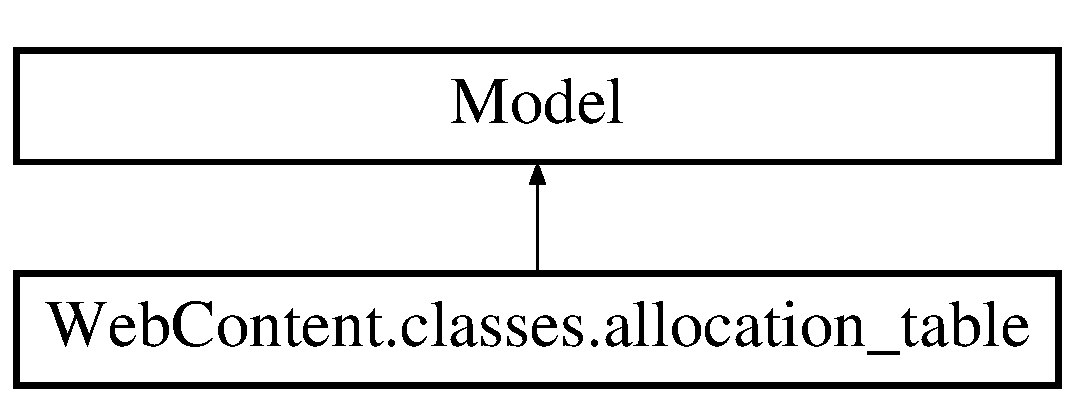
\includegraphics[height=2.000000cm]{class_web_content_1_1classes_1_1allocation__table}
\end{center}
\end{figure}
\subsection*{Public Member Functions}
\begin{DoxyCompactItemize}
\item 
def \hyperlink{class_web_content_1_1classes_1_1allocation__table_a1eecb55816c97b0cb5e07a170289695b}{\+\_\+\+\_\+init\+\_\+\+\_\+} (self, \hyperlink{class_web_content_1_1classes_1_1allocation__table_aa3e71cab5ccef034cc859f9df77b83cb}{idallocation\+\_\+table}, \hyperlink{class_web_content_1_1classes_1_1allocation__table_a22afd1f2474fcb3a8add213aa82f08b9}{name}, \hyperlink{class_web_content_1_1classes_1_1allocation__table_ad98336114a772790e5c148f397de445c}{items\+\_\+id}, \hyperlink{class_web_content_1_1classes_1_1allocation__table_a42be6ad06e7d48d95d6f792d42e44ff6}{user}, \hyperlink{class_web_content_1_1classes_1_1allocation__table_a2e89ec86c3716d18e305c9c259f86eca}{id\+\_\+\+Shows}, \hyperlink{class_web_content_1_1classes_1_1allocation__table_a18854e8abdc8f618ce03cfbfbb0932e8}{quantity}, \hyperlink{class_web_content_1_1classes_1_1allocation__table_a5144b48dae04c952fa2a83701424dee5}{start\+\_\+date}, \hyperlink{class_web_content_1_1classes_1_1allocation__table_a7e1a1a4c7faa7f0af957407a80becd67}{end\+\_\+date}, \hyperlink{class_web_content_1_1classes_1_1allocation__table_a03a6731faa9d3420c8c018cdefbddbb8}{Barcoded}, \hyperlink{class_web_content_1_1classes_1_1allocation__table_a3f9c6c91b93e0802e156df425ba39eba}{quantity\+\_\+available})
\item 
def \hyperlink{class_web_content_1_1classes_1_1allocation__table_ad9d19b4d3ee1752e1d450e50eb34e117}{find\+\_\+quantity} (cls, \hyperlink{class_web_content_1_1classes_1_1allocation__table_ad98336114a772790e5c148f397de445c}{items\+\_\+id}, items\+List)
\end{DoxyCompactItemize}
\subsection*{Static Public Attributes}
\begin{DoxyCompactItemize}
\item 
\hyperlink{class_web_content_1_1classes_1_1allocation__table_aa3e71cab5ccef034cc859f9df77b83cb}{idallocation\+\_\+table} = db.\+Column(\char`\"{}idallocation\+\_\+table\char`\"{}, db.\+Integer, primary\+\_\+key=True)
\item 
\hyperlink{class_web_content_1_1classes_1_1allocation__table_a22afd1f2474fcb3a8add213aa82f08b9}{name} = db.\+Column(\char`\"{}name\char`\"{}, db.\+String(45))
\item 
\hyperlink{class_web_content_1_1classes_1_1allocation__table_ad98336114a772790e5c148f397de445c}{items\+\_\+id} = db.\+Column(\char`\"{}items\+\_\+id\char`\"{}, db.\+Integer)
\item 
\hyperlink{class_web_content_1_1classes_1_1allocation__table_a42be6ad06e7d48d95d6f792d42e44ff6}{user} = db.\+Column(\char`\"{}user\char`\"{}, db.\+String(45))
\item 
\hyperlink{class_web_content_1_1classes_1_1allocation__table_a2e89ec86c3716d18e305c9c259f86eca}{id\+\_\+\+Shows} = db.\+Column(\char`\"{}id\+\_\+\+Shows\char`\"{}, db.\+Integer)
\item 
\hyperlink{class_web_content_1_1classes_1_1allocation__table_a18854e8abdc8f618ce03cfbfbb0932e8}{quantity} = db.\+Column(\char`\"{}quantity\char`\"{}, db.\+Integer)
\item 
\hyperlink{class_web_content_1_1classes_1_1allocation__table_a5144b48dae04c952fa2a83701424dee5}{start\+\_\+date} = db.\+Column(\char`\"{}start\+\_\+date\char`\"{}, db.\+Date\+Time)
\item 
\hyperlink{class_web_content_1_1classes_1_1allocation__table_a7e1a1a4c7faa7f0af957407a80becd67}{end\+\_\+date} = db.\+Column(\char`\"{}end\+\_\+date\char`\"{}, db.\+Date\+Time)
\item 
\hyperlink{class_web_content_1_1classes_1_1allocation__table_a03a6731faa9d3420c8c018cdefbddbb8}{Barcoded} = db.\+Column(\char`\"{}Barcoded\char`\"{}, db.\+String(45))
\item 
\hyperlink{class_web_content_1_1classes_1_1allocation__table_a3f9c6c91b93e0802e156df425ba39eba}{quantity\+\_\+available} = db.\+Column(\char`\"{}quantity\+\_\+available\char`\"{}, db.\+Integer)
\end{DoxyCompactItemize}


\subsection{Detailed Description}


Definition at line 160 of file classes.\+py.



\subsection{Constructor \& Destructor Documentation}
\mbox{\Hypertarget{class_web_content_1_1classes_1_1allocation__table_a1eecb55816c97b0cb5e07a170289695b}\label{class_web_content_1_1classes_1_1allocation__table_a1eecb55816c97b0cb5e07a170289695b}} 
\index{Web\+Content\+::classes\+::allocation\+\_\+table@{Web\+Content\+::classes\+::allocation\+\_\+table}!\+\_\+\+\_\+init\+\_\+\+\_\+@{\+\_\+\+\_\+init\+\_\+\+\_\+}}
\index{\+\_\+\+\_\+init\+\_\+\+\_\+@{\+\_\+\+\_\+init\+\_\+\+\_\+}!Web\+Content\+::classes\+::allocation\+\_\+table@{Web\+Content\+::classes\+::allocation\+\_\+table}}
\subsubsection{\texorpdfstring{\+\_\+\+\_\+init\+\_\+\+\_\+()}{\_\_init\_\_()}}
{\footnotesize\ttfamily def Web\+Content.\+classes.\+allocation\+\_\+table.\+\_\+\+\_\+init\+\_\+\+\_\+ (\begin{DoxyParamCaption}\item[{}]{self,  }\item[{}]{idallocation\+\_\+table,  }\item[{}]{name,  }\item[{}]{items\+\_\+id,  }\item[{}]{user,  }\item[{}]{id\+\_\+\+Shows,  }\item[{}]{quantity,  }\item[{}]{start\+\_\+date,  }\item[{}]{end\+\_\+date,  }\item[{}]{Barcoded,  }\item[{}]{quantity\+\_\+available }\end{DoxyParamCaption})}



Definition at line 173 of file classes.\+py.



\subsection{Member Function Documentation}
\mbox{\Hypertarget{class_web_content_1_1classes_1_1allocation__table_ad9d19b4d3ee1752e1d450e50eb34e117}\label{class_web_content_1_1classes_1_1allocation__table_ad9d19b4d3ee1752e1d450e50eb34e117}} 
\index{Web\+Content\+::classes\+::allocation\+\_\+table@{Web\+Content\+::classes\+::allocation\+\_\+table}!find\+\_\+quantity@{find\+\_\+quantity}}
\index{find\+\_\+quantity@{find\+\_\+quantity}!Web\+Content\+::classes\+::allocation\+\_\+table@{Web\+Content\+::classes\+::allocation\+\_\+table}}
\subsubsection{\texorpdfstring{find\+\_\+quantity()}{find\_quantity()}}
{\footnotesize\ttfamily def Web\+Content.\+classes.\+allocation\+\_\+table.\+find\+\_\+quantity (\begin{DoxyParamCaption}\item[{}]{cls,  }\item[{}]{items\+\_\+id,  }\item[{}]{items\+List }\end{DoxyParamCaption})}



Definition at line 186 of file classes.\+py.



\subsection{Member Data Documentation}
\mbox{\Hypertarget{class_web_content_1_1classes_1_1allocation__table_a03a6731faa9d3420c8c018cdefbddbb8}\label{class_web_content_1_1classes_1_1allocation__table_a03a6731faa9d3420c8c018cdefbddbb8}} 
\index{Web\+Content\+::classes\+::allocation\+\_\+table@{Web\+Content\+::classes\+::allocation\+\_\+table}!Barcoded@{Barcoded}}
\index{Barcoded@{Barcoded}!Web\+Content\+::classes\+::allocation\+\_\+table@{Web\+Content\+::classes\+::allocation\+\_\+table}}
\subsubsection{\texorpdfstring{Barcoded}{Barcoded}}
{\footnotesize\ttfamily Web\+Content.\+classes.\+allocation\+\_\+table.\+Barcoded = db.\+Column(\char`\"{}Barcoded\char`\"{}, db.\+String(45))\hspace{0.3cm}{\ttfamily [static]}}



Definition at line 170 of file classes.\+py.

\mbox{\Hypertarget{class_web_content_1_1classes_1_1allocation__table_a7e1a1a4c7faa7f0af957407a80becd67}\label{class_web_content_1_1classes_1_1allocation__table_a7e1a1a4c7faa7f0af957407a80becd67}} 
\index{Web\+Content\+::classes\+::allocation\+\_\+table@{Web\+Content\+::classes\+::allocation\+\_\+table}!end\+\_\+date@{end\+\_\+date}}
\index{end\+\_\+date@{end\+\_\+date}!Web\+Content\+::classes\+::allocation\+\_\+table@{Web\+Content\+::classes\+::allocation\+\_\+table}}
\subsubsection{\texorpdfstring{end\+\_\+date}{end\_date}}
{\footnotesize\ttfamily Web\+Content.\+classes.\+allocation\+\_\+table.\+end\+\_\+date = db.\+Column(\char`\"{}end\+\_\+date\char`\"{}, db.\+Date\+Time)\hspace{0.3cm}{\ttfamily [static]}}



Definition at line 169 of file classes.\+py.

\mbox{\Hypertarget{class_web_content_1_1classes_1_1allocation__table_a2e89ec86c3716d18e305c9c259f86eca}\label{class_web_content_1_1classes_1_1allocation__table_a2e89ec86c3716d18e305c9c259f86eca}} 
\index{Web\+Content\+::classes\+::allocation\+\_\+table@{Web\+Content\+::classes\+::allocation\+\_\+table}!id\+\_\+\+Shows@{id\+\_\+\+Shows}}
\index{id\+\_\+\+Shows@{id\+\_\+\+Shows}!Web\+Content\+::classes\+::allocation\+\_\+table@{Web\+Content\+::classes\+::allocation\+\_\+table}}
\subsubsection{\texorpdfstring{id\+\_\+\+Shows}{id\_Shows}}
{\footnotesize\ttfamily Web\+Content.\+classes.\+allocation\+\_\+table.\+id\+\_\+\+Shows = db.\+Column(\char`\"{}id\+\_\+\+Shows\char`\"{}, db.\+Integer)\hspace{0.3cm}{\ttfamily [static]}}



Definition at line 166 of file classes.\+py.

\mbox{\Hypertarget{class_web_content_1_1classes_1_1allocation__table_aa3e71cab5ccef034cc859f9df77b83cb}\label{class_web_content_1_1classes_1_1allocation__table_aa3e71cab5ccef034cc859f9df77b83cb}} 
\index{Web\+Content\+::classes\+::allocation\+\_\+table@{Web\+Content\+::classes\+::allocation\+\_\+table}!idallocation\+\_\+table@{idallocation\+\_\+table}}
\index{idallocation\+\_\+table@{idallocation\+\_\+table}!Web\+Content\+::classes\+::allocation\+\_\+table@{Web\+Content\+::classes\+::allocation\+\_\+table}}
\subsubsection{\texorpdfstring{idallocation\+\_\+table}{idallocation\_table}}
{\footnotesize\ttfamily Web\+Content.\+classes.\+allocation\+\_\+table.\+idallocation\+\_\+table = db.\+Column(\char`\"{}idallocation\+\_\+table\char`\"{}, db.\+Integer, primary\+\_\+key=True)\hspace{0.3cm}{\ttfamily [static]}}



Definition at line 162 of file classes.\+py.

\mbox{\Hypertarget{class_web_content_1_1classes_1_1allocation__table_ad98336114a772790e5c148f397de445c}\label{class_web_content_1_1classes_1_1allocation__table_ad98336114a772790e5c148f397de445c}} 
\index{Web\+Content\+::classes\+::allocation\+\_\+table@{Web\+Content\+::classes\+::allocation\+\_\+table}!items\+\_\+id@{items\+\_\+id}}
\index{items\+\_\+id@{items\+\_\+id}!Web\+Content\+::classes\+::allocation\+\_\+table@{Web\+Content\+::classes\+::allocation\+\_\+table}}
\subsubsection{\texorpdfstring{items\+\_\+id}{items\_id}}
{\footnotesize\ttfamily Web\+Content.\+classes.\+allocation\+\_\+table.\+items\+\_\+id = db.\+Column(\char`\"{}items\+\_\+id\char`\"{}, db.\+Integer)\hspace{0.3cm}{\ttfamily [static]}}



Definition at line 164 of file classes.\+py.

\mbox{\Hypertarget{class_web_content_1_1classes_1_1allocation__table_a22afd1f2474fcb3a8add213aa82f08b9}\label{class_web_content_1_1classes_1_1allocation__table_a22afd1f2474fcb3a8add213aa82f08b9}} 
\index{Web\+Content\+::classes\+::allocation\+\_\+table@{Web\+Content\+::classes\+::allocation\+\_\+table}!name@{name}}
\index{name@{name}!Web\+Content\+::classes\+::allocation\+\_\+table@{Web\+Content\+::classes\+::allocation\+\_\+table}}
\subsubsection{\texorpdfstring{name}{name}}
{\footnotesize\ttfamily Web\+Content.\+classes.\+allocation\+\_\+table.\+name = db.\+Column(\char`\"{}name\char`\"{}, db.\+String(45))\hspace{0.3cm}{\ttfamily [static]}}



Definition at line 163 of file classes.\+py.

\mbox{\Hypertarget{class_web_content_1_1classes_1_1allocation__table_a18854e8abdc8f618ce03cfbfbb0932e8}\label{class_web_content_1_1classes_1_1allocation__table_a18854e8abdc8f618ce03cfbfbb0932e8}} 
\index{Web\+Content\+::classes\+::allocation\+\_\+table@{Web\+Content\+::classes\+::allocation\+\_\+table}!quantity@{quantity}}
\index{quantity@{quantity}!Web\+Content\+::classes\+::allocation\+\_\+table@{Web\+Content\+::classes\+::allocation\+\_\+table}}
\subsubsection{\texorpdfstring{quantity}{quantity}}
{\footnotesize\ttfamily Web\+Content.\+classes.\+allocation\+\_\+table.\+quantity = db.\+Column(\char`\"{}quantity\char`\"{}, db.\+Integer)\hspace{0.3cm}{\ttfamily [static]}}



Definition at line 167 of file classes.\+py.

\mbox{\Hypertarget{class_web_content_1_1classes_1_1allocation__table_a3f9c6c91b93e0802e156df425ba39eba}\label{class_web_content_1_1classes_1_1allocation__table_a3f9c6c91b93e0802e156df425ba39eba}} 
\index{Web\+Content\+::classes\+::allocation\+\_\+table@{Web\+Content\+::classes\+::allocation\+\_\+table}!quantity\+\_\+available@{quantity\+\_\+available}}
\index{quantity\+\_\+available@{quantity\+\_\+available}!Web\+Content\+::classes\+::allocation\+\_\+table@{Web\+Content\+::classes\+::allocation\+\_\+table}}
\subsubsection{\texorpdfstring{quantity\+\_\+available}{quantity\_available}}
{\footnotesize\ttfamily Web\+Content.\+classes.\+allocation\+\_\+table.\+quantity\+\_\+available = db.\+Column(\char`\"{}quantity\+\_\+available\char`\"{}, db.\+Integer)\hspace{0.3cm}{\ttfamily [static]}}



Definition at line 171 of file classes.\+py.

\mbox{\Hypertarget{class_web_content_1_1classes_1_1allocation__table_a5144b48dae04c952fa2a83701424dee5}\label{class_web_content_1_1classes_1_1allocation__table_a5144b48dae04c952fa2a83701424dee5}} 
\index{Web\+Content\+::classes\+::allocation\+\_\+table@{Web\+Content\+::classes\+::allocation\+\_\+table}!start\+\_\+date@{start\+\_\+date}}
\index{start\+\_\+date@{start\+\_\+date}!Web\+Content\+::classes\+::allocation\+\_\+table@{Web\+Content\+::classes\+::allocation\+\_\+table}}
\subsubsection{\texorpdfstring{start\+\_\+date}{start\_date}}
{\footnotesize\ttfamily Web\+Content.\+classes.\+allocation\+\_\+table.\+start\+\_\+date = db.\+Column(\char`\"{}start\+\_\+date\char`\"{}, db.\+Date\+Time)\hspace{0.3cm}{\ttfamily [static]}}



Definition at line 168 of file classes.\+py.

\mbox{\Hypertarget{class_web_content_1_1classes_1_1allocation__table_a42be6ad06e7d48d95d6f792d42e44ff6}\label{class_web_content_1_1classes_1_1allocation__table_a42be6ad06e7d48d95d6f792d42e44ff6}} 
\index{Web\+Content\+::classes\+::allocation\+\_\+table@{Web\+Content\+::classes\+::allocation\+\_\+table}!user@{user}}
\index{user@{user}!Web\+Content\+::classes\+::allocation\+\_\+table@{Web\+Content\+::classes\+::allocation\+\_\+table}}
\subsubsection{\texorpdfstring{user}{user}}
{\footnotesize\ttfamily Web\+Content.\+classes.\+allocation\+\_\+table.\+user = db.\+Column(\char`\"{}user\char`\"{}, db.\+String(45))\hspace{0.3cm}{\ttfamily [static]}}



Definition at line 165 of file classes.\+py.



The documentation for this class was generated from the following file\+:\begin{DoxyCompactItemize}
\item 
C\+:/\+Users/\+Antonio/\+Documents/\+Git\+Hub/\+Spitfire\+Capstone/\+Web\+Content/\hyperlink{classes_8py}{classes.\+py}\end{DoxyCompactItemize}

\hypertarget{class_web_content_1_1classes_1_1contacts}{}\section{Web\+Content.\+classes.\+contacts Class Reference}
\label{class_web_content_1_1classes_1_1contacts}\index{Web\+Content.\+classes.\+contacts@{Web\+Content.\+classes.\+contacts}}
Inheritance diagram for Web\+Content.\+classes.\+contacts\+:\begin{figure}[H]
\begin{center}
\leavevmode
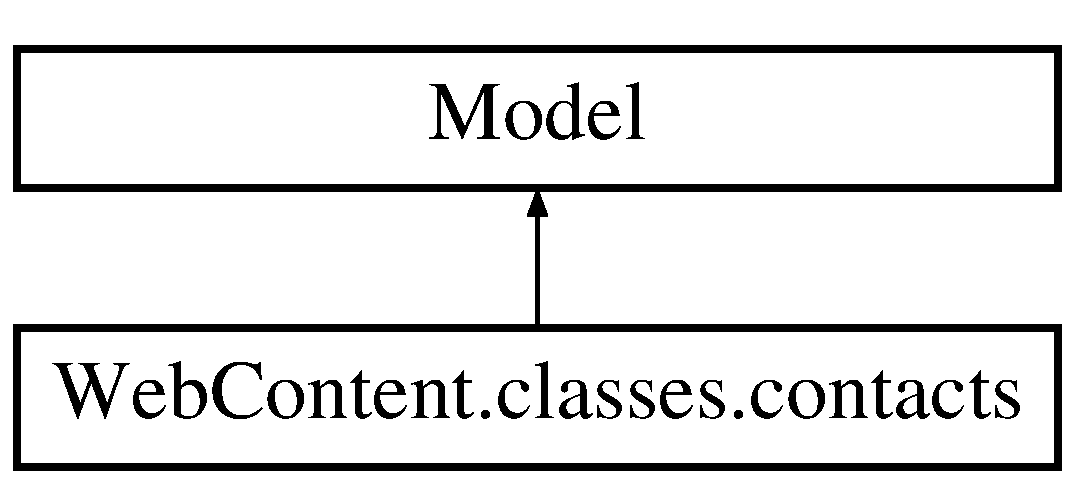
\includegraphics[height=2.000000cm]{class_web_content_1_1classes_1_1contacts}
\end{center}
\end{figure}
\subsection*{Public Member Functions}
\begin{DoxyCompactItemize}
\item 
def \hyperlink{class_web_content_1_1classes_1_1contacts_a867bb2313c6cc01e6d3fa6936257f70c}{\+\_\+\+\_\+init\+\_\+\+\_\+} (self, \hyperlink{class_web_content_1_1classes_1_1contacts_af5b7ebdde96128f644dba2c9003395e1}{contact\+Name}, \hyperlink{class_web_content_1_1classes_1_1contacts_aa2f4eaf4a9e2620d3f9cf92d359cb68e}{contact\+Address}, \hyperlink{class_web_content_1_1classes_1_1contacts_ab337e819e9708c4385d88e19e5b4272a}{contact\+City}, \hyperlink{class_web_content_1_1classes_1_1contacts_aff779f52e8d69185e09157ab38bbeef2}{contact\+Zip}, \hyperlink{class_web_content_1_1classes_1_1contacts_aa4c26f3a90e573a3d5495dd9fea09067}{Phone}, \hyperlink{class_web_content_1_1classes_1_1contacts_af308c0c25a34db25695da939142548da}{Email}, \hyperlink{class_web_content_1_1classes_1_1contacts_a6ef2db0009b3b8b0facfaf88d54b84e1}{is\+Employee})
\item 
def \hyperlink{class_web_content_1_1classes_1_1contacts_a7d04c296ef51af2cfc29faa3a8ee9e3a}{\+\_\+\+\_\+repr\+\_\+\+\_\+} (self)
\end{DoxyCompactItemize}
\subsection*{Static Public Attributes}
\begin{DoxyCompactItemize}
\item 
\hyperlink{class_web_content_1_1classes_1_1contacts_af5b7ebdde96128f644dba2c9003395e1}{contact\+Name} = db.\+Column(\textquotesingle{}contact\+Name\textquotesingle{}, db.\+String(55), primary\+\_\+key=True)
\item 
\hyperlink{class_web_content_1_1classes_1_1contacts_aa2f4eaf4a9e2620d3f9cf92d359cb68e}{contact\+Address} = db.\+Column(\textquotesingle{}contact\+Address\textquotesingle{}, db.\+String(55))
\item 
\hyperlink{class_web_content_1_1classes_1_1contacts_ab337e819e9708c4385d88e19e5b4272a}{contact\+City} = db.\+Column(\textquotesingle{}contact\+City\textquotesingle{}, db.\+String(45))
\item 
\hyperlink{class_web_content_1_1classes_1_1contacts_aff779f52e8d69185e09157ab38bbeef2}{contact\+Zip} = db.\+Column(\textquotesingle{}contact\+Zip\textquotesingle{}, db.\+Integer)
\item 
\hyperlink{class_web_content_1_1classes_1_1contacts_aa4c26f3a90e573a3d5495dd9fea09067}{Phone} = db.\+Column(\textquotesingle{}Phone\textquotesingle{}, db.\+String(14))
\item 
\hyperlink{class_web_content_1_1classes_1_1contacts_af308c0c25a34db25695da939142548da}{Email} = db.\+Column(\textquotesingle{}Email\textquotesingle{}, db.\+String(255))
\item 
\hyperlink{class_web_content_1_1classes_1_1contacts_a6ef2db0009b3b8b0facfaf88d54b84e1}{is\+Employee} = db.\+Column(\textquotesingle{}is\+Employee\textquotesingle{}, db.\+String(1))
\end{DoxyCompactItemize}


\subsection{Constructor \& Destructor Documentation}
\mbox{\Hypertarget{class_web_content_1_1classes_1_1contacts_a867bb2313c6cc01e6d3fa6936257f70c}\label{class_web_content_1_1classes_1_1contacts_a867bb2313c6cc01e6d3fa6936257f70c}} 
\index{Web\+Content\+::classes\+::contacts@{Web\+Content\+::classes\+::contacts}!\+\_\+\+\_\+init\+\_\+\+\_\+@{\+\_\+\+\_\+init\+\_\+\+\_\+}}
\index{\+\_\+\+\_\+init\+\_\+\+\_\+@{\+\_\+\+\_\+init\+\_\+\+\_\+}!Web\+Content\+::classes\+::contacts@{Web\+Content\+::classes\+::contacts}}
\subsubsection{\texorpdfstring{\+\_\+\+\_\+init\+\_\+\+\_\+()}{\_\_init\_\_()}}
{\footnotesize\ttfamily def Web\+Content.\+classes.\+contacts.\+\_\+\+\_\+init\+\_\+\+\_\+ (\begin{DoxyParamCaption}\item[{}]{self,  }\item[{}]{contact\+Name,  }\item[{}]{contact\+Address,  }\item[{}]{contact\+City,  }\item[{}]{contact\+Zip,  }\item[{}]{Phone,  }\item[{}]{Email,  }\item[{}]{is\+Employee }\end{DoxyParamCaption})}



\subsection{Member Function Documentation}
\mbox{\Hypertarget{class_web_content_1_1classes_1_1contacts_a7d04c296ef51af2cfc29faa3a8ee9e3a}\label{class_web_content_1_1classes_1_1contacts_a7d04c296ef51af2cfc29faa3a8ee9e3a}} 
\index{Web\+Content\+::classes\+::contacts@{Web\+Content\+::classes\+::contacts}!\+\_\+\+\_\+repr\+\_\+\+\_\+@{\+\_\+\+\_\+repr\+\_\+\+\_\+}}
\index{\+\_\+\+\_\+repr\+\_\+\+\_\+@{\+\_\+\+\_\+repr\+\_\+\+\_\+}!Web\+Content\+::classes\+::contacts@{Web\+Content\+::classes\+::contacts}}
\subsubsection{\texorpdfstring{\+\_\+\+\_\+repr\+\_\+\+\_\+()}{\_\_repr\_\_()}}
{\footnotesize\ttfamily def Web\+Content.\+classes.\+contacts.\+\_\+\+\_\+repr\+\_\+\+\_\+ (\begin{DoxyParamCaption}\item[{}]{self }\end{DoxyParamCaption})}



\subsection{Member Data Documentation}
\mbox{\Hypertarget{class_web_content_1_1classes_1_1contacts_aa2f4eaf4a9e2620d3f9cf92d359cb68e}\label{class_web_content_1_1classes_1_1contacts_aa2f4eaf4a9e2620d3f9cf92d359cb68e}} 
\index{Web\+Content\+::classes\+::contacts@{Web\+Content\+::classes\+::contacts}!contact\+Address@{contact\+Address}}
\index{contact\+Address@{contact\+Address}!Web\+Content\+::classes\+::contacts@{Web\+Content\+::classes\+::contacts}}
\subsubsection{\texorpdfstring{contact\+Address}{contactAddress}}
{\footnotesize\ttfamily Web\+Content.\+classes.\+contacts.\+contact\+Address = db.\+Column(\textquotesingle{}contact\+Address\textquotesingle{}, db.\+String(55))\hspace{0.3cm}{\ttfamily [static]}}

\mbox{\Hypertarget{class_web_content_1_1classes_1_1contacts_ab337e819e9708c4385d88e19e5b4272a}\label{class_web_content_1_1classes_1_1contacts_ab337e819e9708c4385d88e19e5b4272a}} 
\index{Web\+Content\+::classes\+::contacts@{Web\+Content\+::classes\+::contacts}!contact\+City@{contact\+City}}
\index{contact\+City@{contact\+City}!Web\+Content\+::classes\+::contacts@{Web\+Content\+::classes\+::contacts}}
\subsubsection{\texorpdfstring{contact\+City}{contactCity}}
{\footnotesize\ttfamily Web\+Content.\+classes.\+contacts.\+contact\+City = db.\+Column(\textquotesingle{}contact\+City\textquotesingle{}, db.\+String(45))\hspace{0.3cm}{\ttfamily [static]}}

\mbox{\Hypertarget{class_web_content_1_1classes_1_1contacts_af5b7ebdde96128f644dba2c9003395e1}\label{class_web_content_1_1classes_1_1contacts_af5b7ebdde96128f644dba2c9003395e1}} 
\index{Web\+Content\+::classes\+::contacts@{Web\+Content\+::classes\+::contacts}!contact\+Name@{contact\+Name}}
\index{contact\+Name@{contact\+Name}!Web\+Content\+::classes\+::contacts@{Web\+Content\+::classes\+::contacts}}
\subsubsection{\texorpdfstring{contact\+Name}{contactName}}
{\footnotesize\ttfamily Web\+Content.\+classes.\+contacts.\+contact\+Name = db.\+Column(\textquotesingle{}contact\+Name\textquotesingle{}, db.\+String(55), primary\+\_\+key=True)\hspace{0.3cm}{\ttfamily [static]}}

\mbox{\Hypertarget{class_web_content_1_1classes_1_1contacts_aff779f52e8d69185e09157ab38bbeef2}\label{class_web_content_1_1classes_1_1contacts_aff779f52e8d69185e09157ab38bbeef2}} 
\index{Web\+Content\+::classes\+::contacts@{Web\+Content\+::classes\+::contacts}!contact\+Zip@{contact\+Zip}}
\index{contact\+Zip@{contact\+Zip}!Web\+Content\+::classes\+::contacts@{Web\+Content\+::classes\+::contacts}}
\subsubsection{\texorpdfstring{contact\+Zip}{contactZip}}
{\footnotesize\ttfamily Web\+Content.\+classes.\+contacts.\+contact\+Zip = db.\+Column(\textquotesingle{}contact\+Zip\textquotesingle{}, db.\+Integer)\hspace{0.3cm}{\ttfamily [static]}}

\mbox{\Hypertarget{class_web_content_1_1classes_1_1contacts_af308c0c25a34db25695da939142548da}\label{class_web_content_1_1classes_1_1contacts_af308c0c25a34db25695da939142548da}} 
\index{Web\+Content\+::classes\+::contacts@{Web\+Content\+::classes\+::contacts}!Email@{Email}}
\index{Email@{Email}!Web\+Content\+::classes\+::contacts@{Web\+Content\+::classes\+::contacts}}
\subsubsection{\texorpdfstring{Email}{Email}}
{\footnotesize\ttfamily Web\+Content.\+classes.\+contacts.\+Email = db.\+Column(\textquotesingle{}Email\textquotesingle{}, db.\+String(255))\hspace{0.3cm}{\ttfamily [static]}}

\mbox{\Hypertarget{class_web_content_1_1classes_1_1contacts_a6ef2db0009b3b8b0facfaf88d54b84e1}\label{class_web_content_1_1classes_1_1contacts_a6ef2db0009b3b8b0facfaf88d54b84e1}} 
\index{Web\+Content\+::classes\+::contacts@{Web\+Content\+::classes\+::contacts}!is\+Employee@{is\+Employee}}
\index{is\+Employee@{is\+Employee}!Web\+Content\+::classes\+::contacts@{Web\+Content\+::classes\+::contacts}}
\subsubsection{\texorpdfstring{is\+Employee}{isEmployee}}
{\footnotesize\ttfamily Web\+Content.\+classes.\+contacts.\+is\+Employee = db.\+Column(\textquotesingle{}is\+Employee\textquotesingle{}, db.\+String(1))\hspace{0.3cm}{\ttfamily [static]}}

\mbox{\Hypertarget{class_web_content_1_1classes_1_1contacts_aa4c26f3a90e573a3d5495dd9fea09067}\label{class_web_content_1_1classes_1_1contacts_aa4c26f3a90e573a3d5495dd9fea09067}} 
\index{Web\+Content\+::classes\+::contacts@{Web\+Content\+::classes\+::contacts}!Phone@{Phone}}
\index{Phone@{Phone}!Web\+Content\+::classes\+::contacts@{Web\+Content\+::classes\+::contacts}}
\subsubsection{\texorpdfstring{Phone}{Phone}}
{\footnotesize\ttfamily Web\+Content.\+classes.\+contacts.\+Phone = db.\+Column(\textquotesingle{}Phone\textquotesingle{}, db.\+String(14))\hspace{0.3cm}{\ttfamily [static]}}



The documentation for this class was generated from the following file\+:\begin{DoxyCompactItemize}
\item 
\hyperlink{classes_8py}{classes.\+py}\end{DoxyCompactItemize}

\hypertarget{class_web_content_1_1classes_1_1daily__task}{}\section{Web\+Content.\+classes.\+daily\+\_\+task Class Reference}
\label{class_web_content_1_1classes_1_1daily__task}\index{Web\+Content.\+classes.\+daily\+\_\+task@{Web\+Content.\+classes.\+daily\+\_\+task}}
Inheritance diagram for Web\+Content.\+classes.\+daily\+\_\+task\+:\begin{figure}[H]
\begin{center}
\leavevmode
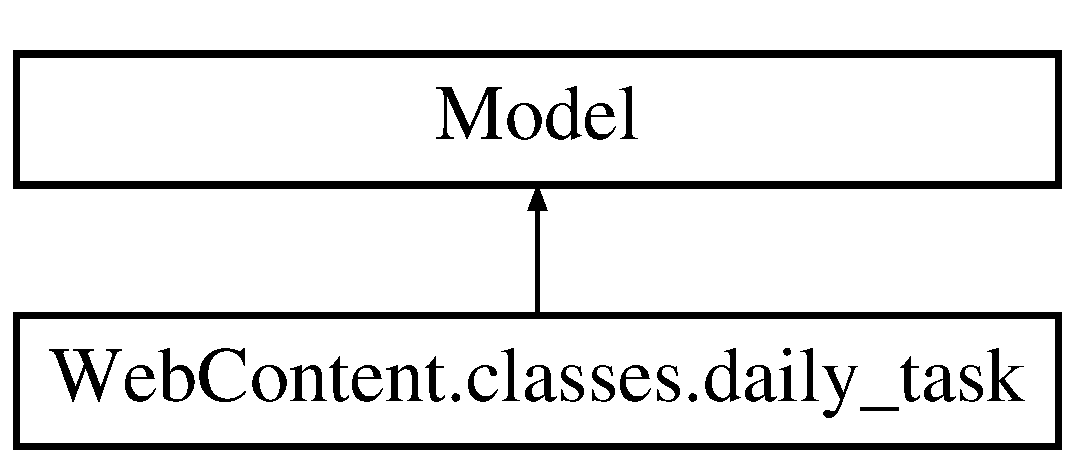
\includegraphics[height=2.000000cm]{class_web_content_1_1classes_1_1daily__task}
\end{center}
\end{figure}
\subsection*{Public Member Functions}
\begin{DoxyCompactItemize}
\item 
def \hyperlink{class_web_content_1_1classes_1_1daily__task_ad42f8d2b69ae7b520baf2ff107d412dd}{\+\_\+\+\_\+init\+\_\+\+\_\+} (self, \hyperlink{class_web_content_1_1classes_1_1daily__task_a16bbcb32784e7dce04634c70d657d17d}{iddaily\+\_\+task}, \hyperlink{class_web_content_1_1classes_1_1daily__task_aafd4c49d7d757e26f13bf61a4e6aa875}{task}, \hyperlink{class_web_content_1_1classes_1_1daily__task_acd856b954382e792e6e5c28fd830121e}{place}, \hyperlink{class_web_content_1_1classes_1_1daily__task_a8adebd433b814a8e63ddff8c74dec3ae}{note}, \hyperlink{class_web_content_1_1classes_1_1daily__task_ad2c51b720cec786c89d5742e03b240ca}{time}, \hyperlink{class_web_content_1_1classes_1_1daily__task_a3d81a54b4ec50f7b09a5c9a7126e1b91}{date})
\item 
def \hyperlink{class_web_content_1_1classes_1_1daily__task_aceb8f58140226c7c645ecd7d75f875bd}{\+\_\+\+\_\+repr\+\_\+\+\_\+} (self)
\end{DoxyCompactItemize}
\subsection*{Static Public Attributes}
\begin{DoxyCompactItemize}
\item 
\hyperlink{class_web_content_1_1classes_1_1daily__task_a16bbcb32784e7dce04634c70d657d17d}{iddaily\+\_\+task} = db.\+Column(\char`\"{}iddaily\+\_\+task\char`\"{}, db.\+String(50), primary\+\_\+key=True)
\item 
\hyperlink{class_web_content_1_1classes_1_1daily__task_aafd4c49d7d757e26f13bf61a4e6aa875}{task} = db.\+Column(\char`\"{}task\char`\"{}, db.\+String(50))
\item 
\hyperlink{class_web_content_1_1classes_1_1daily__task_acd856b954382e792e6e5c28fd830121e}{place} = db.\+Column(\char`\"{}place\char`\"{}, db.\+String(50))
\item 
\hyperlink{class_web_content_1_1classes_1_1daily__task_a8adebd433b814a8e63ddff8c74dec3ae}{note} = db.\+Column(\char`\"{}note\char`\"{}, db.\+String(50))
\item 
\hyperlink{class_web_content_1_1classes_1_1daily__task_ad2c51b720cec786c89d5742e03b240ca}{time} = db.\+Column(\char`\"{}time\char`\"{}, db.\+String(10))
\item 
\hyperlink{class_web_content_1_1classes_1_1daily__task_a3d81a54b4ec50f7b09a5c9a7126e1b91}{date} = db.\+Column(\char`\"{}date\char`\"{}, db.\+String(15))
\end{DoxyCompactItemize}


\subsection{Detailed Description}


Definition at line 196 of file classes.\+py.



\subsection{Constructor \& Destructor Documentation}
\mbox{\Hypertarget{class_web_content_1_1classes_1_1daily__task_ad42f8d2b69ae7b520baf2ff107d412dd}\label{class_web_content_1_1classes_1_1daily__task_ad42f8d2b69ae7b520baf2ff107d412dd}} 
\index{Web\+Content\+::classes\+::daily\+\_\+task@{Web\+Content\+::classes\+::daily\+\_\+task}!\+\_\+\+\_\+init\+\_\+\+\_\+@{\+\_\+\+\_\+init\+\_\+\+\_\+}}
\index{\+\_\+\+\_\+init\+\_\+\+\_\+@{\+\_\+\+\_\+init\+\_\+\+\_\+}!Web\+Content\+::classes\+::daily\+\_\+task@{Web\+Content\+::classes\+::daily\+\_\+task}}
\subsubsection{\texorpdfstring{\+\_\+\+\_\+init\+\_\+\+\_\+()}{\_\_init\_\_()}}
{\footnotesize\ttfamily def Web\+Content.\+classes.\+daily\+\_\+task.\+\_\+\+\_\+init\+\_\+\+\_\+ (\begin{DoxyParamCaption}\item[{}]{self,  }\item[{}]{iddaily\+\_\+task,  }\item[{}]{task,  }\item[{}]{place,  }\item[{}]{note,  }\item[{}]{time,  }\item[{}]{date }\end{DoxyParamCaption})}



Definition at line 205 of file classes.\+py.



\subsection{Member Function Documentation}
\mbox{\Hypertarget{class_web_content_1_1classes_1_1daily__task_aceb8f58140226c7c645ecd7d75f875bd}\label{class_web_content_1_1classes_1_1daily__task_aceb8f58140226c7c645ecd7d75f875bd}} 
\index{Web\+Content\+::classes\+::daily\+\_\+task@{Web\+Content\+::classes\+::daily\+\_\+task}!\+\_\+\+\_\+repr\+\_\+\+\_\+@{\+\_\+\+\_\+repr\+\_\+\+\_\+}}
\index{\+\_\+\+\_\+repr\+\_\+\+\_\+@{\+\_\+\+\_\+repr\+\_\+\+\_\+}!Web\+Content\+::classes\+::daily\+\_\+task@{Web\+Content\+::classes\+::daily\+\_\+task}}
\subsubsection{\texorpdfstring{\+\_\+\+\_\+repr\+\_\+\+\_\+()}{\_\_repr\_\_()}}
{\footnotesize\ttfamily def Web\+Content.\+classes.\+daily\+\_\+task.\+\_\+\+\_\+repr\+\_\+\+\_\+ (\begin{DoxyParamCaption}\item[{}]{self }\end{DoxyParamCaption})}



Definition at line 213 of file classes.\+py.



\subsection{Member Data Documentation}
\mbox{\Hypertarget{class_web_content_1_1classes_1_1daily__task_a3d81a54b4ec50f7b09a5c9a7126e1b91}\label{class_web_content_1_1classes_1_1daily__task_a3d81a54b4ec50f7b09a5c9a7126e1b91}} 
\index{Web\+Content\+::classes\+::daily\+\_\+task@{Web\+Content\+::classes\+::daily\+\_\+task}!date@{date}}
\index{date@{date}!Web\+Content\+::classes\+::daily\+\_\+task@{Web\+Content\+::classes\+::daily\+\_\+task}}
\subsubsection{\texorpdfstring{date}{date}}
{\footnotesize\ttfamily Web\+Content.\+classes.\+daily\+\_\+task.\+date = db.\+Column(\char`\"{}date\char`\"{}, db.\+String(15))\hspace{0.3cm}{\ttfamily [static]}}



Definition at line 203 of file classes.\+py.

\mbox{\Hypertarget{class_web_content_1_1classes_1_1daily__task_a16bbcb32784e7dce04634c70d657d17d}\label{class_web_content_1_1classes_1_1daily__task_a16bbcb32784e7dce04634c70d657d17d}} 
\index{Web\+Content\+::classes\+::daily\+\_\+task@{Web\+Content\+::classes\+::daily\+\_\+task}!iddaily\+\_\+task@{iddaily\+\_\+task}}
\index{iddaily\+\_\+task@{iddaily\+\_\+task}!Web\+Content\+::classes\+::daily\+\_\+task@{Web\+Content\+::classes\+::daily\+\_\+task}}
\subsubsection{\texorpdfstring{iddaily\+\_\+task}{iddaily\_task}}
{\footnotesize\ttfamily Web\+Content.\+classes.\+daily\+\_\+task.\+iddaily\+\_\+task = db.\+Column(\char`\"{}iddaily\+\_\+task\char`\"{}, db.\+String(50), primary\+\_\+key=True)\hspace{0.3cm}{\ttfamily [static]}}



Definition at line 198 of file classes.\+py.

\mbox{\Hypertarget{class_web_content_1_1classes_1_1daily__task_a8adebd433b814a8e63ddff8c74dec3ae}\label{class_web_content_1_1classes_1_1daily__task_a8adebd433b814a8e63ddff8c74dec3ae}} 
\index{Web\+Content\+::classes\+::daily\+\_\+task@{Web\+Content\+::classes\+::daily\+\_\+task}!note@{note}}
\index{note@{note}!Web\+Content\+::classes\+::daily\+\_\+task@{Web\+Content\+::classes\+::daily\+\_\+task}}
\subsubsection{\texorpdfstring{note}{note}}
{\footnotesize\ttfamily Web\+Content.\+classes.\+daily\+\_\+task.\+note = db.\+Column(\char`\"{}note\char`\"{}, db.\+String(50))\hspace{0.3cm}{\ttfamily [static]}}



Definition at line 201 of file classes.\+py.

\mbox{\Hypertarget{class_web_content_1_1classes_1_1daily__task_acd856b954382e792e6e5c28fd830121e}\label{class_web_content_1_1classes_1_1daily__task_acd856b954382e792e6e5c28fd830121e}} 
\index{Web\+Content\+::classes\+::daily\+\_\+task@{Web\+Content\+::classes\+::daily\+\_\+task}!place@{place}}
\index{place@{place}!Web\+Content\+::classes\+::daily\+\_\+task@{Web\+Content\+::classes\+::daily\+\_\+task}}
\subsubsection{\texorpdfstring{place}{place}}
{\footnotesize\ttfamily Web\+Content.\+classes.\+daily\+\_\+task.\+place = db.\+Column(\char`\"{}place\char`\"{}, db.\+String(50))\hspace{0.3cm}{\ttfamily [static]}}



Definition at line 200 of file classes.\+py.

\mbox{\Hypertarget{class_web_content_1_1classes_1_1daily__task_aafd4c49d7d757e26f13bf61a4e6aa875}\label{class_web_content_1_1classes_1_1daily__task_aafd4c49d7d757e26f13bf61a4e6aa875}} 
\index{Web\+Content\+::classes\+::daily\+\_\+task@{Web\+Content\+::classes\+::daily\+\_\+task}!task@{task}}
\index{task@{task}!Web\+Content\+::classes\+::daily\+\_\+task@{Web\+Content\+::classes\+::daily\+\_\+task}}
\subsubsection{\texorpdfstring{task}{task}}
{\footnotesize\ttfamily Web\+Content.\+classes.\+daily\+\_\+task.\+task = db.\+Column(\char`\"{}task\char`\"{}, db.\+String(50))\hspace{0.3cm}{\ttfamily [static]}}



Definition at line 199 of file classes.\+py.

\mbox{\Hypertarget{class_web_content_1_1classes_1_1daily__task_ad2c51b720cec786c89d5742e03b240ca}\label{class_web_content_1_1classes_1_1daily__task_ad2c51b720cec786c89d5742e03b240ca}} 
\index{Web\+Content\+::classes\+::daily\+\_\+task@{Web\+Content\+::classes\+::daily\+\_\+task}!time@{time}}
\index{time@{time}!Web\+Content\+::classes\+::daily\+\_\+task@{Web\+Content\+::classes\+::daily\+\_\+task}}
\subsubsection{\texorpdfstring{time}{time}}
{\footnotesize\ttfamily Web\+Content.\+classes.\+daily\+\_\+task.\+time = db.\+Column(\char`\"{}time\char`\"{}, db.\+String(10))\hspace{0.3cm}{\ttfamily [static]}}



Definition at line 202 of file classes.\+py.



The documentation for this class was generated from the following file\+:\begin{DoxyCompactItemize}
\item 
C\+:/\+Users/\+Antonio/\+Documents/\+Git\+Hub/\+Spitfire\+Capstone/\+Web\+Content/\hyperlink{classes_8py}{classes.\+py}\end{DoxyCompactItemize}

\hypertarget{class_web_content_1_1classes_1_1items}{}\section{Web\+Content.\+classes.\+items Class Reference}
\label{class_web_content_1_1classes_1_1items}\index{Web\+Content.\+classes.\+items@{Web\+Content.\+classes.\+items}}
Inheritance diagram for Web\+Content.\+classes.\+items\+:\begin{figure}[H]
\begin{center}
\leavevmode
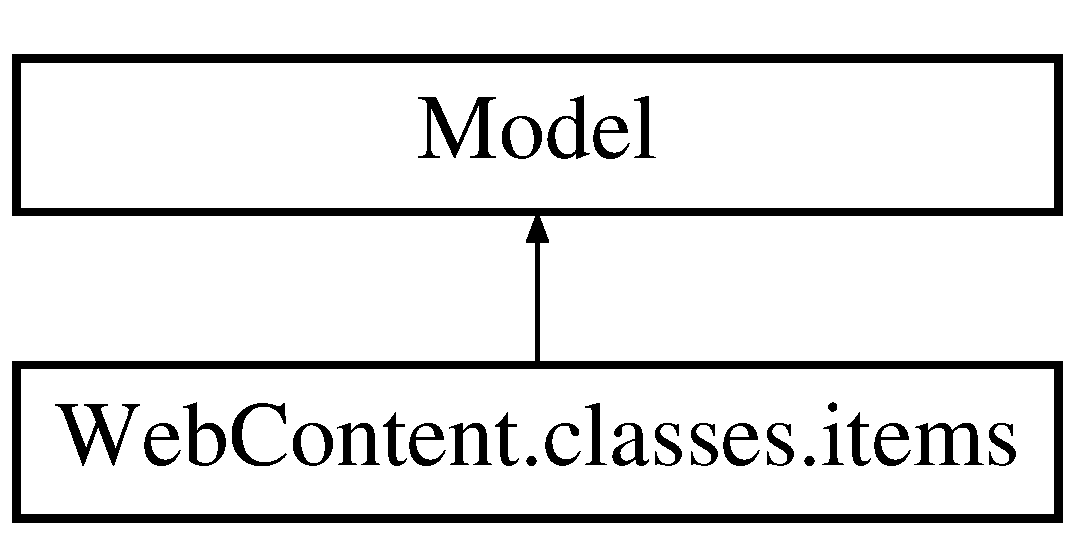
\includegraphics[height=2.000000cm]{class_web_content_1_1classes_1_1items}
\end{center}
\end{figure}
\subsection*{Public Member Functions}
\begin{DoxyCompactItemize}
\item 
def \hyperlink{class_web_content_1_1classes_1_1items_a69e23b8eb679a8f5fe127d05368f146c}{\+\_\+\+\_\+init\+\_\+\+\_\+} (self, \hyperlink{class_web_content_1_1classes_1_1items_ae81c7aff4b6699e4b73fdc2c58e7c17f}{id\+Items}, \hyperlink{class_web_content_1_1classes_1_1items_a6b9cc2755a793d5710d6aaa583c64ed7}{name}, \hyperlink{class_web_content_1_1classes_1_1items_ad3adf84b02910cbad246217c240b9bc1}{quantity}, \hyperlink{class_web_content_1_1classes_1_1items_a921e7c462d24e352af1c6386e33d4a54}{mastercategory}, \hyperlink{class_web_content_1_1classes_1_1items_abf504f02bb8165be106746d68ea6500a}{subcategory}, \hyperlink{class_web_content_1_1classes_1_1items_a84d35b34ce8cd95db165e325ce94f043}{pictures}, \hyperlink{class_web_content_1_1classes_1_1items_a0b093c44310dcd97c97580ef744ab1cd}{code})
\item 
def \hyperlink{class_web_content_1_1classes_1_1items_af090fcd951f16fc9e653dd0ca161dbcb}{\+\_\+\+\_\+repr\+\_\+\+\_\+} (self)
\end{DoxyCompactItemize}
\subsection*{Static Public Attributes}
\begin{DoxyCompactItemize}
\item 
\hyperlink{class_web_content_1_1classes_1_1items_ae81c7aff4b6699e4b73fdc2c58e7c17f}{id\+Items} = db.\+Column(\textquotesingle{}id\+Items\textquotesingle{}, db.\+Integer, primary\+\_\+key=True)
\item 
\hyperlink{class_web_content_1_1classes_1_1items_a6b9cc2755a793d5710d6aaa583c64ed7}{name} = db.\+Column(\textquotesingle{}name\textquotesingle{}, db.\+String(45))
\item 
\hyperlink{class_web_content_1_1classes_1_1items_ad3adf84b02910cbad246217c240b9bc1}{quantity} = db.\+Column(\textquotesingle{}quantity\textquotesingle{}, db.\+Integer)
\item 
\hyperlink{class_web_content_1_1classes_1_1items_a921e7c462d24e352af1c6386e33d4a54}{mastercategory} = db.\+Column(\textquotesingle{}master\+\_\+category\textquotesingle{}, db.\+String(45))
\item 
\hyperlink{class_web_content_1_1classes_1_1items_abf504f02bb8165be106746d68ea6500a}{subcategory} = db.\+Column(\textquotesingle{}sub\+\_\+category\textquotesingle{}, db.\+String(45))
\item 
\hyperlink{class_web_content_1_1classes_1_1items_a84d35b34ce8cd95db165e325ce94f043}{pictures} = db.\+Column(\textquotesingle{}pictures\textquotesingle{}, db.\+String(45))
\item 
\hyperlink{class_web_content_1_1classes_1_1items_a0b093c44310dcd97c97580ef744ab1cd}{code} = db.\+Column(\textquotesingle{}code\textquotesingle{}, db.\+String(45))
\end{DoxyCompactItemize}


\subsection{Detailed Description}


Definition at line 25 of file classes.\+py.



\subsection{Constructor \& Destructor Documentation}
\mbox{\Hypertarget{class_web_content_1_1classes_1_1items_a69e23b8eb679a8f5fe127d05368f146c}\label{class_web_content_1_1classes_1_1items_a69e23b8eb679a8f5fe127d05368f146c}} 
\index{Web\+Content\+::classes\+::items@{Web\+Content\+::classes\+::items}!\+\_\+\+\_\+init\+\_\+\+\_\+@{\+\_\+\+\_\+init\+\_\+\+\_\+}}
\index{\+\_\+\+\_\+init\+\_\+\+\_\+@{\+\_\+\+\_\+init\+\_\+\+\_\+}!Web\+Content\+::classes\+::items@{Web\+Content\+::classes\+::items}}
\subsubsection{\texorpdfstring{\+\_\+\+\_\+init\+\_\+\+\_\+()}{\_\_init\_\_()}}
{\footnotesize\ttfamily def Web\+Content.\+classes.\+items.\+\_\+\+\_\+init\+\_\+\+\_\+ (\begin{DoxyParamCaption}\item[{}]{self,  }\item[{}]{id\+Items,  }\item[{}]{name,  }\item[{}]{quantity,  }\item[{}]{mastercategory,  }\item[{}]{subcategory,  }\item[{}]{pictures,  }\item[{}]{code }\end{DoxyParamCaption})}



Definition at line 35 of file classes.\+py.



\subsection{Member Function Documentation}
\mbox{\Hypertarget{class_web_content_1_1classes_1_1items_af090fcd951f16fc9e653dd0ca161dbcb}\label{class_web_content_1_1classes_1_1items_af090fcd951f16fc9e653dd0ca161dbcb}} 
\index{Web\+Content\+::classes\+::items@{Web\+Content\+::classes\+::items}!\+\_\+\+\_\+repr\+\_\+\+\_\+@{\+\_\+\+\_\+repr\+\_\+\+\_\+}}
\index{\+\_\+\+\_\+repr\+\_\+\+\_\+@{\+\_\+\+\_\+repr\+\_\+\+\_\+}!Web\+Content\+::classes\+::items@{Web\+Content\+::classes\+::items}}
\subsubsection{\texorpdfstring{\+\_\+\+\_\+repr\+\_\+\+\_\+()}{\_\_repr\_\_()}}
{\footnotesize\ttfamily def Web\+Content.\+classes.\+items.\+\_\+\+\_\+repr\+\_\+\+\_\+ (\begin{DoxyParamCaption}\item[{}]{self }\end{DoxyParamCaption})}



Definition at line 44 of file classes.\+py.



\subsection{Member Data Documentation}
\mbox{\Hypertarget{class_web_content_1_1classes_1_1items_a0b093c44310dcd97c97580ef744ab1cd}\label{class_web_content_1_1classes_1_1items_a0b093c44310dcd97c97580ef744ab1cd}} 
\index{Web\+Content\+::classes\+::items@{Web\+Content\+::classes\+::items}!code@{code}}
\index{code@{code}!Web\+Content\+::classes\+::items@{Web\+Content\+::classes\+::items}}
\subsubsection{\texorpdfstring{code}{code}}
{\footnotesize\ttfamily Web\+Content.\+classes.\+items.\+code = db.\+Column(\textquotesingle{}code\textquotesingle{}, db.\+String(45))\hspace{0.3cm}{\ttfamily [static]}}



Definition at line 33 of file classes.\+py.

\mbox{\Hypertarget{class_web_content_1_1classes_1_1items_ae81c7aff4b6699e4b73fdc2c58e7c17f}\label{class_web_content_1_1classes_1_1items_ae81c7aff4b6699e4b73fdc2c58e7c17f}} 
\index{Web\+Content\+::classes\+::items@{Web\+Content\+::classes\+::items}!id\+Items@{id\+Items}}
\index{id\+Items@{id\+Items}!Web\+Content\+::classes\+::items@{Web\+Content\+::classes\+::items}}
\subsubsection{\texorpdfstring{id\+Items}{idItems}}
{\footnotesize\ttfamily Web\+Content.\+classes.\+items.\+id\+Items = db.\+Column(\textquotesingle{}id\+Items\textquotesingle{}, db.\+Integer, primary\+\_\+key=True)\hspace{0.3cm}{\ttfamily [static]}}



Definition at line 27 of file classes.\+py.

\mbox{\Hypertarget{class_web_content_1_1classes_1_1items_a921e7c462d24e352af1c6386e33d4a54}\label{class_web_content_1_1classes_1_1items_a921e7c462d24e352af1c6386e33d4a54}} 
\index{Web\+Content\+::classes\+::items@{Web\+Content\+::classes\+::items}!mastercategory@{mastercategory}}
\index{mastercategory@{mastercategory}!Web\+Content\+::classes\+::items@{Web\+Content\+::classes\+::items}}
\subsubsection{\texorpdfstring{mastercategory}{mastercategory}}
{\footnotesize\ttfamily Web\+Content.\+classes.\+items.\+mastercategory = db.\+Column(\textquotesingle{}master\+\_\+category\textquotesingle{}, db.\+String(45))\hspace{0.3cm}{\ttfamily [static]}}



Definition at line 30 of file classes.\+py.

\mbox{\Hypertarget{class_web_content_1_1classes_1_1items_a6b9cc2755a793d5710d6aaa583c64ed7}\label{class_web_content_1_1classes_1_1items_a6b9cc2755a793d5710d6aaa583c64ed7}} 
\index{Web\+Content\+::classes\+::items@{Web\+Content\+::classes\+::items}!name@{name}}
\index{name@{name}!Web\+Content\+::classes\+::items@{Web\+Content\+::classes\+::items}}
\subsubsection{\texorpdfstring{name}{name}}
{\footnotesize\ttfamily Web\+Content.\+classes.\+items.\+name = db.\+Column(\textquotesingle{}name\textquotesingle{}, db.\+String(45))\hspace{0.3cm}{\ttfamily [static]}}



Definition at line 28 of file classes.\+py.

\mbox{\Hypertarget{class_web_content_1_1classes_1_1items_a84d35b34ce8cd95db165e325ce94f043}\label{class_web_content_1_1classes_1_1items_a84d35b34ce8cd95db165e325ce94f043}} 
\index{Web\+Content\+::classes\+::items@{Web\+Content\+::classes\+::items}!pictures@{pictures}}
\index{pictures@{pictures}!Web\+Content\+::classes\+::items@{Web\+Content\+::classes\+::items}}
\subsubsection{\texorpdfstring{pictures}{pictures}}
{\footnotesize\ttfamily Web\+Content.\+classes.\+items.\+pictures = db.\+Column(\textquotesingle{}pictures\textquotesingle{}, db.\+String(45))\hspace{0.3cm}{\ttfamily [static]}}



Definition at line 32 of file classes.\+py.

\mbox{\Hypertarget{class_web_content_1_1classes_1_1items_ad3adf84b02910cbad246217c240b9bc1}\label{class_web_content_1_1classes_1_1items_ad3adf84b02910cbad246217c240b9bc1}} 
\index{Web\+Content\+::classes\+::items@{Web\+Content\+::classes\+::items}!quantity@{quantity}}
\index{quantity@{quantity}!Web\+Content\+::classes\+::items@{Web\+Content\+::classes\+::items}}
\subsubsection{\texorpdfstring{quantity}{quantity}}
{\footnotesize\ttfamily Web\+Content.\+classes.\+items.\+quantity = db.\+Column(\textquotesingle{}quantity\textquotesingle{}, db.\+Integer)\hspace{0.3cm}{\ttfamily [static]}}



Definition at line 29 of file classes.\+py.

\mbox{\Hypertarget{class_web_content_1_1classes_1_1items_abf504f02bb8165be106746d68ea6500a}\label{class_web_content_1_1classes_1_1items_abf504f02bb8165be106746d68ea6500a}} 
\index{Web\+Content\+::classes\+::items@{Web\+Content\+::classes\+::items}!subcategory@{subcategory}}
\index{subcategory@{subcategory}!Web\+Content\+::classes\+::items@{Web\+Content\+::classes\+::items}}
\subsubsection{\texorpdfstring{subcategory}{subcategory}}
{\footnotesize\ttfamily Web\+Content.\+classes.\+items.\+subcategory = db.\+Column(\textquotesingle{}sub\+\_\+category\textquotesingle{}, db.\+String(45))\hspace{0.3cm}{\ttfamily [static]}}



Definition at line 31 of file classes.\+py.



The documentation for this class was generated from the following file\+:\begin{DoxyCompactItemize}
\item 
C\+:/\+Users/\+Antonio/\+Documents/\+Git\+Hub/\+Spitfire\+Capstone/\+Web\+Content/\hyperlink{classes_8py}{classes.\+py}\end{DoxyCompactItemize}

\hypertarget{class_web_content_1_1classes_1_1job_gear}{}\section{Web\+Content.\+classes.\+job\+Gear Class Reference}
\label{class_web_content_1_1classes_1_1job_gear}\index{Web\+Content.\+classes.\+job\+Gear@{Web\+Content.\+classes.\+job\+Gear}}
Inheritance diagram for Web\+Content.\+classes.\+job\+Gear\+:\begin{figure}[H]
\begin{center}
\leavevmode
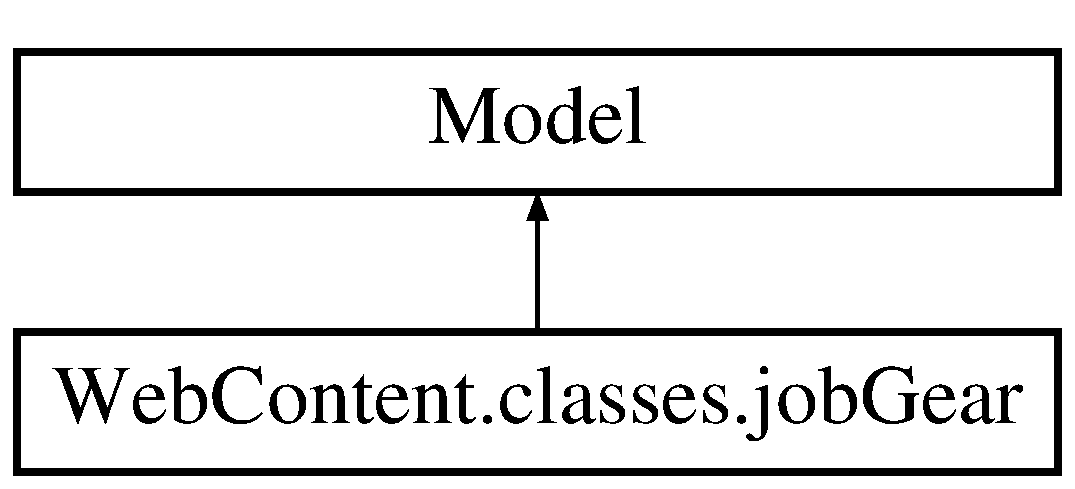
\includegraphics[height=2.000000cm]{class_web_content_1_1classes_1_1job_gear}
\end{center}
\end{figure}
\subsection*{Public Member Functions}
\begin{DoxyCompactItemize}
\item 
def \hyperlink{class_web_content_1_1classes_1_1job_gear_a65e8cf098ecea70db55ad9bd0a3639e2}{\+\_\+\+\_\+init\+\_\+\+\_\+} (self, \hyperlink{class_web_content_1_1classes_1_1job_gear_a3c06d5a64cb18ce600a7e015d7ad7e2e}{id\+Items}, \hyperlink{class_web_content_1_1classes_1_1job_gear_ac24ca34d6bcaedda98f1711e0733c8ed}{Name}, \hyperlink{class_web_content_1_1classes_1_1job_gear_ad4f9a871b8c10bcdc1e3921b313620ca}{Quantity}, \hyperlink{class_web_content_1_1classes_1_1job_gear_aa99b6c99df4ef2686d9a7ae05839e870}{Barcode}, \hyperlink{class_web_content_1_1classes_1_1job_gear_ac60ca08b7517caefae54fd99e8c2f854}{show})
\item 
def \hyperlink{class_web_content_1_1classes_1_1job_gear_a366770b8baf200be438b1a6d5bebf72b}{\+\_\+\+\_\+repr\+\_\+\+\_\+} (self)
\end{DoxyCompactItemize}
\subsection*{Static Public Attributes}
\begin{DoxyCompactItemize}
\item 
\hyperlink{class_web_content_1_1classes_1_1job_gear_a3c06d5a64cb18ce600a7e015d7ad7e2e}{id\+Items} = db.\+Column(\textquotesingle{}id\+Items\textquotesingle{}, db.\+Integer, primary\+\_\+key=True)
\item 
\hyperlink{class_web_content_1_1classes_1_1job_gear_ac24ca34d6bcaedda98f1711e0733c8ed}{Name} = db.\+Column(\textquotesingle{}Name\textquotesingle{}, db.\+String(45))
\item 
\hyperlink{class_web_content_1_1classes_1_1job_gear_ad4f9a871b8c10bcdc1e3921b313620ca}{Quantity} = db.\+Column(\textquotesingle{}Quantity\textquotesingle{}, db.\+Integer)
\item 
\hyperlink{class_web_content_1_1classes_1_1job_gear_aa99b6c99df4ef2686d9a7ae05839e870}{Barcode} = db.\+Column(\textquotesingle{}Barcode\textquotesingle{}, db.\+String(45))
\item 
\hyperlink{class_web_content_1_1classes_1_1job_gear_ac60ca08b7517caefae54fd99e8c2f854}{show} = db.\+Column(\textquotesingle{}show\textquotesingle{}, db.\+String(45))
\end{DoxyCompactItemize}


\subsection{Constructor \& Destructor Documentation}
\mbox{\Hypertarget{class_web_content_1_1classes_1_1job_gear_a65e8cf098ecea70db55ad9bd0a3639e2}\label{class_web_content_1_1classes_1_1job_gear_a65e8cf098ecea70db55ad9bd0a3639e2}} 
\index{Web\+Content\+::classes\+::job\+Gear@{Web\+Content\+::classes\+::job\+Gear}!\+\_\+\+\_\+init\+\_\+\+\_\+@{\+\_\+\+\_\+init\+\_\+\+\_\+}}
\index{\+\_\+\+\_\+init\+\_\+\+\_\+@{\+\_\+\+\_\+init\+\_\+\+\_\+}!Web\+Content\+::classes\+::job\+Gear@{Web\+Content\+::classes\+::job\+Gear}}
\subsubsection{\texorpdfstring{\+\_\+\+\_\+init\+\_\+\+\_\+()}{\_\_init\_\_()}}
{\footnotesize\ttfamily def Web\+Content.\+classes.\+job\+Gear.\+\_\+\+\_\+init\+\_\+\+\_\+ (\begin{DoxyParamCaption}\item[{}]{self,  }\item[{}]{id\+Items,  }\item[{}]{Name,  }\item[{}]{Quantity,  }\item[{}]{Barcode,  }\item[{}]{show }\end{DoxyParamCaption})}



\subsection{Member Function Documentation}
\mbox{\Hypertarget{class_web_content_1_1classes_1_1job_gear_a366770b8baf200be438b1a6d5bebf72b}\label{class_web_content_1_1classes_1_1job_gear_a366770b8baf200be438b1a6d5bebf72b}} 
\index{Web\+Content\+::classes\+::job\+Gear@{Web\+Content\+::classes\+::job\+Gear}!\+\_\+\+\_\+repr\+\_\+\+\_\+@{\+\_\+\+\_\+repr\+\_\+\+\_\+}}
\index{\+\_\+\+\_\+repr\+\_\+\+\_\+@{\+\_\+\+\_\+repr\+\_\+\+\_\+}!Web\+Content\+::classes\+::job\+Gear@{Web\+Content\+::classes\+::job\+Gear}}
\subsubsection{\texorpdfstring{\+\_\+\+\_\+repr\+\_\+\+\_\+()}{\_\_repr\_\_()}}
{\footnotesize\ttfamily def Web\+Content.\+classes.\+job\+Gear.\+\_\+\+\_\+repr\+\_\+\+\_\+ (\begin{DoxyParamCaption}\item[{}]{self }\end{DoxyParamCaption})}



\subsection{Member Data Documentation}
\mbox{\Hypertarget{class_web_content_1_1classes_1_1job_gear_aa99b6c99df4ef2686d9a7ae05839e870}\label{class_web_content_1_1classes_1_1job_gear_aa99b6c99df4ef2686d9a7ae05839e870}} 
\index{Web\+Content\+::classes\+::job\+Gear@{Web\+Content\+::classes\+::job\+Gear}!Barcode@{Barcode}}
\index{Barcode@{Barcode}!Web\+Content\+::classes\+::job\+Gear@{Web\+Content\+::classes\+::job\+Gear}}
\subsubsection{\texorpdfstring{Barcode}{Barcode}}
{\footnotesize\ttfamily Web\+Content.\+classes.\+job\+Gear.\+Barcode = db.\+Column(\textquotesingle{}Barcode\textquotesingle{}, db.\+String(45))\hspace{0.3cm}{\ttfamily [static]}}

\mbox{\Hypertarget{class_web_content_1_1classes_1_1job_gear_a3c06d5a64cb18ce600a7e015d7ad7e2e}\label{class_web_content_1_1classes_1_1job_gear_a3c06d5a64cb18ce600a7e015d7ad7e2e}} 
\index{Web\+Content\+::classes\+::job\+Gear@{Web\+Content\+::classes\+::job\+Gear}!id\+Items@{id\+Items}}
\index{id\+Items@{id\+Items}!Web\+Content\+::classes\+::job\+Gear@{Web\+Content\+::classes\+::job\+Gear}}
\subsubsection{\texorpdfstring{id\+Items}{idItems}}
{\footnotesize\ttfamily Web\+Content.\+classes.\+job\+Gear.\+id\+Items = db.\+Column(\textquotesingle{}id\+Items\textquotesingle{}, db.\+Integer, primary\+\_\+key=True)\hspace{0.3cm}{\ttfamily [static]}}

\mbox{\Hypertarget{class_web_content_1_1classes_1_1job_gear_ac24ca34d6bcaedda98f1711e0733c8ed}\label{class_web_content_1_1classes_1_1job_gear_ac24ca34d6bcaedda98f1711e0733c8ed}} 
\index{Web\+Content\+::classes\+::job\+Gear@{Web\+Content\+::classes\+::job\+Gear}!Name@{Name}}
\index{Name@{Name}!Web\+Content\+::classes\+::job\+Gear@{Web\+Content\+::classes\+::job\+Gear}}
\subsubsection{\texorpdfstring{Name}{Name}}
{\footnotesize\ttfamily Web\+Content.\+classes.\+job\+Gear.\+Name = db.\+Column(\textquotesingle{}Name\textquotesingle{}, db.\+String(45))\hspace{0.3cm}{\ttfamily [static]}}

\mbox{\Hypertarget{class_web_content_1_1classes_1_1job_gear_ad4f9a871b8c10bcdc1e3921b313620ca}\label{class_web_content_1_1classes_1_1job_gear_ad4f9a871b8c10bcdc1e3921b313620ca}} 
\index{Web\+Content\+::classes\+::job\+Gear@{Web\+Content\+::classes\+::job\+Gear}!Quantity@{Quantity}}
\index{Quantity@{Quantity}!Web\+Content\+::classes\+::job\+Gear@{Web\+Content\+::classes\+::job\+Gear}}
\subsubsection{\texorpdfstring{Quantity}{Quantity}}
{\footnotesize\ttfamily Web\+Content.\+classes.\+job\+Gear.\+Quantity = db.\+Column(\textquotesingle{}Quantity\textquotesingle{}, db.\+Integer)\hspace{0.3cm}{\ttfamily [static]}}

\mbox{\Hypertarget{class_web_content_1_1classes_1_1job_gear_ac60ca08b7517caefae54fd99e8c2f854}\label{class_web_content_1_1classes_1_1job_gear_ac60ca08b7517caefae54fd99e8c2f854}} 
\index{Web\+Content\+::classes\+::job\+Gear@{Web\+Content\+::classes\+::job\+Gear}!show@{show}}
\index{show@{show}!Web\+Content\+::classes\+::job\+Gear@{Web\+Content\+::classes\+::job\+Gear}}
\subsubsection{\texorpdfstring{show}{show}}
{\footnotesize\ttfamily Web\+Content.\+classes.\+job\+Gear.\+show = db.\+Column(\textquotesingle{}show\textquotesingle{}, db.\+String(45))\hspace{0.3cm}{\ttfamily [static]}}



The documentation for this class was generated from the following file\+:\begin{DoxyCompactItemize}
\item 
\hyperlink{classes_8py}{classes.\+py}\end{DoxyCompactItemize}

\hypertarget{class_web_content_1_1classes_1_1_shows}{}\section{Web\+Content.\+classes.\+Shows Class Reference}
\label{class_web_content_1_1classes_1_1_shows}\index{Web\+Content.\+classes.\+Shows@{Web\+Content.\+classes.\+Shows}}
Inheritance diagram for Web\+Content.\+classes.\+Shows\+:\begin{figure}[H]
\begin{center}
\leavevmode
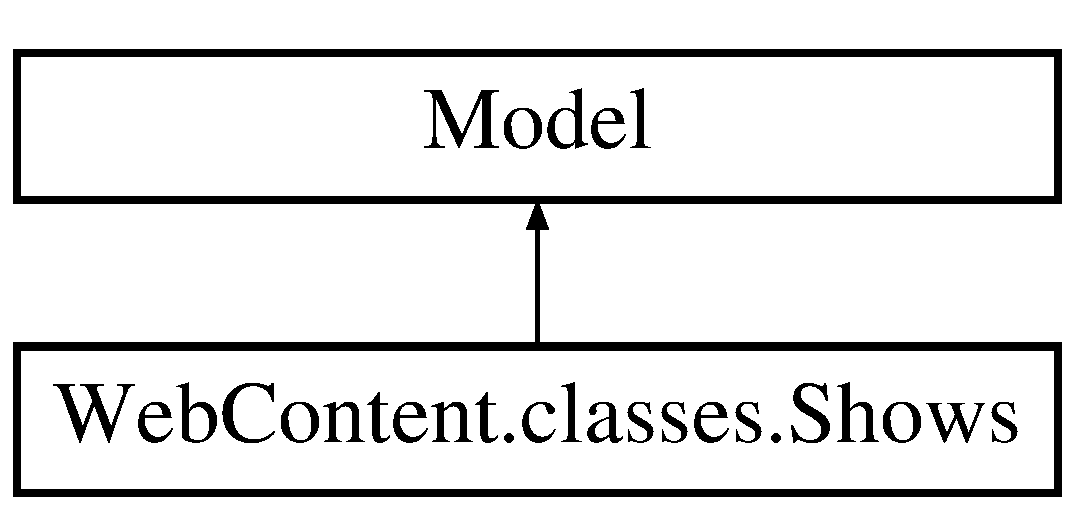
\includegraphics[height=2.000000cm]{class_web_content_1_1classes_1_1_shows}
\end{center}
\end{figure}
\subsection*{Public Member Functions}
\begin{DoxyCompactItemize}
\item 
def \hyperlink{class_web_content_1_1classes_1_1_shows_aa08b1c685aa53cfa043340f94e63905e}{\+\_\+\+\_\+init\+\_\+\+\_\+} (self, \hyperlink{class_web_content_1_1classes_1_1_shows_a9ed1265f6e8a1078de474691f846f793}{id\+Shows}, \hyperlink{class_web_content_1_1classes_1_1_shows_aec2efee9bcdad6b3a4732d6327d7f25c}{show}, \hyperlink{class_web_content_1_1classes_1_1_shows_a6c17ca935d1ab7bce12c2ad5a55bfd0e}{start\+\_\+date}, \hyperlink{class_web_content_1_1classes_1_1_shows_a8e22ab3d1b30b350f3464bcd61b3ab8a}{end\+\_\+date}, \hyperlink{class_web_content_1_1classes_1_1_shows_ad70665816e2050b3176e90e95655f3fb}{show\+\_\+start}, \hyperlink{class_web_content_1_1classes_1_1_shows_aee5eee42b3d279a14f401c113d79083c}{return\+\_\+date}, \hyperlink{class_web_content_1_1classes_1_1_shows_ac931bd921ecb35a0e221ff9133162d2c}{venue}, \hyperlink{class_web_content_1_1classes_1_1_shows_ad95c8895e4633584f7da017e2b79f45d}{client}, \hyperlink{class_web_content_1_1classes_1_1_shows_ae5f65ed709a0218f1298610e91500719}{job\+\_\+type}, \hyperlink{class_web_content_1_1classes_1_1_shows_ae116171a1ecb47ad43e5631115fe9f43}{status}, \hyperlink{class_web_content_1_1classes_1_1_shows_a23219663a5b011841e8054fc6ca88e0f}{handler}, \hyperlink{class_web_content_1_1classes_1_1_shows_a59168ff70138cf3bafb49d58bc7e4cbe}{salesperson}, \hyperlink{class_web_content_1_1classes_1_1_shows_a1c11f5ef467e4230b4672c40cd7268fe}{created\+\_\+by})
\item 
def \hyperlink{class_web_content_1_1classes_1_1_shows_a6691b87ec53fa9349d04a41317fd1bee}{\+\_\+\+\_\+repr\+\_\+\+\_\+} (self)
\end{DoxyCompactItemize}
\subsection*{Static Public Attributes}
\begin{DoxyCompactItemize}
\item 
\hyperlink{class_web_content_1_1classes_1_1_shows_a9ed1265f6e8a1078de474691f846f793}{id\+Shows} = db.\+Column(\textquotesingle{}id\+Shows\textquotesingle{}, db.\+Integer, primary\+\_\+key=True)
\item 
\hyperlink{class_web_content_1_1classes_1_1_shows_aec2efee9bcdad6b3a4732d6327d7f25c}{show} = db.\+Column(\textquotesingle{}show\textquotesingle{}, db.\+String(45))
\item 
\hyperlink{class_web_content_1_1classes_1_1_shows_a6c17ca935d1ab7bce12c2ad5a55bfd0e}{start\+\_\+date} = db.\+Column(\textquotesingle{}start\textquotesingle{}, db.\+Date\+Time)
\item 
\hyperlink{class_web_content_1_1classes_1_1_shows_a8e22ab3d1b30b350f3464bcd61b3ab8a}{end\+\_\+date} = db.\+Column(\textquotesingle{}end\textquotesingle{}, db.\+Date\+Time)
\item 
\hyperlink{class_web_content_1_1classes_1_1_shows_ad70665816e2050b3176e90e95655f3fb}{show\+\_\+start} = db.\+Column(\textquotesingle{}show\+\_\+start\textquotesingle{}, db.\+Date\+Time)
\item 
\hyperlink{class_web_content_1_1classes_1_1_shows_aee5eee42b3d279a14f401c113d79083c}{return\+\_\+date} = db.\+Column(\textquotesingle{}return\textquotesingle{}, db.\+Date\+Time)
\item 
\hyperlink{class_web_content_1_1classes_1_1_shows_ac931bd921ecb35a0e221ff9133162d2c}{venue} = db.\+Column(\textquotesingle{}venue\textquotesingle{}, db.\+String(45))
\item 
\hyperlink{class_web_content_1_1classes_1_1_shows_ad95c8895e4633584f7da017e2b79f45d}{client} = db.\+Column(\textquotesingle{}client\textquotesingle{}, db.\+String(45))
\item 
\hyperlink{class_web_content_1_1classes_1_1_shows_ae5f65ed709a0218f1298610e91500719}{job\+\_\+type} = db.\+Column(\textquotesingle{}job\+\_\+type\textquotesingle{}, db.\+String(45))
\item 
\hyperlink{class_web_content_1_1classes_1_1_shows_ae116171a1ecb47ad43e5631115fe9f43}{status} = db.\+Column(\textquotesingle{}status\textquotesingle{}, db.\+String(45))
\item 
\hyperlink{class_web_content_1_1classes_1_1_shows_a23219663a5b011841e8054fc6ca88e0f}{handler} = db.\+Column(\textquotesingle{}handler\textquotesingle{}, db.\+String(45))
\item 
\hyperlink{class_web_content_1_1classes_1_1_shows_a59168ff70138cf3bafb49d58bc7e4cbe}{salesperson} = db.\+Column(\textquotesingle{}salesperson\textquotesingle{}, db.\+String(45))
\item 
\hyperlink{class_web_content_1_1classes_1_1_shows_a1c11f5ef467e4230b4672c40cd7268fe}{created\+\_\+by} = db.\+Column(\textquotesingle{}created\+\_\+by\textquotesingle{}, db.\+String(45))
\end{DoxyCompactItemize}


\subsection{Detailed Description}


Definition at line 48 of file classes.\+py.



\subsection{Constructor \& Destructor Documentation}
\mbox{\Hypertarget{class_web_content_1_1classes_1_1_shows_aa08b1c685aa53cfa043340f94e63905e}\label{class_web_content_1_1classes_1_1_shows_aa08b1c685aa53cfa043340f94e63905e}} 
\index{Web\+Content\+::classes\+::\+Shows@{Web\+Content\+::classes\+::\+Shows}!\+\_\+\+\_\+init\+\_\+\+\_\+@{\+\_\+\+\_\+init\+\_\+\+\_\+}}
\index{\+\_\+\+\_\+init\+\_\+\+\_\+@{\+\_\+\+\_\+init\+\_\+\+\_\+}!Web\+Content\+::classes\+::\+Shows@{Web\+Content\+::classes\+::\+Shows}}
\subsubsection{\texorpdfstring{\+\_\+\+\_\+init\+\_\+\+\_\+()}{\_\_init\_\_()}}
{\footnotesize\ttfamily def Web\+Content.\+classes.\+Shows.\+\_\+\+\_\+init\+\_\+\+\_\+ (\begin{DoxyParamCaption}\item[{}]{self,  }\item[{}]{id\+Shows,  }\item[{}]{show,  }\item[{}]{start\+\_\+date,  }\item[{}]{end\+\_\+date,  }\item[{}]{show\+\_\+start,  }\item[{}]{return\+\_\+date,  }\item[{}]{venue,  }\item[{}]{client,  }\item[{}]{job\+\_\+type,  }\item[{}]{status,  }\item[{}]{handler,  }\item[{}]{salesperson,  }\item[{}]{created\+\_\+by }\end{DoxyParamCaption})}



Definition at line 65 of file classes.\+py.



\subsection{Member Function Documentation}
\mbox{\Hypertarget{class_web_content_1_1classes_1_1_shows_a6691b87ec53fa9349d04a41317fd1bee}\label{class_web_content_1_1classes_1_1_shows_a6691b87ec53fa9349d04a41317fd1bee}} 
\index{Web\+Content\+::classes\+::\+Shows@{Web\+Content\+::classes\+::\+Shows}!\+\_\+\+\_\+repr\+\_\+\+\_\+@{\+\_\+\+\_\+repr\+\_\+\+\_\+}}
\index{\+\_\+\+\_\+repr\+\_\+\+\_\+@{\+\_\+\+\_\+repr\+\_\+\+\_\+}!Web\+Content\+::classes\+::\+Shows@{Web\+Content\+::classes\+::\+Shows}}
\subsubsection{\texorpdfstring{\+\_\+\+\_\+repr\+\_\+\+\_\+()}{\_\_repr\_\_()}}
{\footnotesize\ttfamily def Web\+Content.\+classes.\+Shows.\+\_\+\+\_\+repr\+\_\+\+\_\+ (\begin{DoxyParamCaption}\item[{}]{self }\end{DoxyParamCaption})}



Definition at line 79 of file classes.\+py.



\subsection{Member Data Documentation}
\mbox{\Hypertarget{class_web_content_1_1classes_1_1_shows_ad95c8895e4633584f7da017e2b79f45d}\label{class_web_content_1_1classes_1_1_shows_ad95c8895e4633584f7da017e2b79f45d}} 
\index{Web\+Content\+::classes\+::\+Shows@{Web\+Content\+::classes\+::\+Shows}!client@{client}}
\index{client@{client}!Web\+Content\+::classes\+::\+Shows@{Web\+Content\+::classes\+::\+Shows}}
\subsubsection{\texorpdfstring{client}{client}}
{\footnotesize\ttfamily Web\+Content.\+classes.\+Shows.\+client = db.\+Column(\textquotesingle{}client\textquotesingle{}, db.\+String(45))\hspace{0.3cm}{\ttfamily [static]}}



Definition at line 57 of file classes.\+py.

\mbox{\Hypertarget{class_web_content_1_1classes_1_1_shows_a1c11f5ef467e4230b4672c40cd7268fe}\label{class_web_content_1_1classes_1_1_shows_a1c11f5ef467e4230b4672c40cd7268fe}} 
\index{Web\+Content\+::classes\+::\+Shows@{Web\+Content\+::classes\+::\+Shows}!created\+\_\+by@{created\+\_\+by}}
\index{created\+\_\+by@{created\+\_\+by}!Web\+Content\+::classes\+::\+Shows@{Web\+Content\+::classes\+::\+Shows}}
\subsubsection{\texorpdfstring{created\+\_\+by}{created\_by}}
{\footnotesize\ttfamily Web\+Content.\+classes.\+Shows.\+created\+\_\+by = db.\+Column(\textquotesingle{}created\+\_\+by\textquotesingle{}, db.\+String(45))\hspace{0.3cm}{\ttfamily [static]}}



Definition at line 62 of file classes.\+py.

\mbox{\Hypertarget{class_web_content_1_1classes_1_1_shows_a8e22ab3d1b30b350f3464bcd61b3ab8a}\label{class_web_content_1_1classes_1_1_shows_a8e22ab3d1b30b350f3464bcd61b3ab8a}} 
\index{Web\+Content\+::classes\+::\+Shows@{Web\+Content\+::classes\+::\+Shows}!end\+\_\+date@{end\+\_\+date}}
\index{end\+\_\+date@{end\+\_\+date}!Web\+Content\+::classes\+::\+Shows@{Web\+Content\+::classes\+::\+Shows}}
\subsubsection{\texorpdfstring{end\+\_\+date}{end\_date}}
{\footnotesize\ttfamily Web\+Content.\+classes.\+Shows.\+end\+\_\+date = db.\+Column(\textquotesingle{}end\textquotesingle{}, db.\+Date\+Time)\hspace{0.3cm}{\ttfamily [static]}}



Definition at line 53 of file classes.\+py.

\mbox{\Hypertarget{class_web_content_1_1classes_1_1_shows_a23219663a5b011841e8054fc6ca88e0f}\label{class_web_content_1_1classes_1_1_shows_a23219663a5b011841e8054fc6ca88e0f}} 
\index{Web\+Content\+::classes\+::\+Shows@{Web\+Content\+::classes\+::\+Shows}!handler@{handler}}
\index{handler@{handler}!Web\+Content\+::classes\+::\+Shows@{Web\+Content\+::classes\+::\+Shows}}
\subsubsection{\texorpdfstring{handler}{handler}}
{\footnotesize\ttfamily Web\+Content.\+classes.\+Shows.\+handler = db.\+Column(\textquotesingle{}handler\textquotesingle{}, db.\+String(45))\hspace{0.3cm}{\ttfamily [static]}}



Definition at line 60 of file classes.\+py.

\mbox{\Hypertarget{class_web_content_1_1classes_1_1_shows_a9ed1265f6e8a1078de474691f846f793}\label{class_web_content_1_1classes_1_1_shows_a9ed1265f6e8a1078de474691f846f793}} 
\index{Web\+Content\+::classes\+::\+Shows@{Web\+Content\+::classes\+::\+Shows}!id\+Shows@{id\+Shows}}
\index{id\+Shows@{id\+Shows}!Web\+Content\+::classes\+::\+Shows@{Web\+Content\+::classes\+::\+Shows}}
\subsubsection{\texorpdfstring{id\+Shows}{idShows}}
{\footnotesize\ttfamily Web\+Content.\+classes.\+Shows.\+id\+Shows = db.\+Column(\textquotesingle{}id\+Shows\textquotesingle{}, db.\+Integer, primary\+\_\+key=True)\hspace{0.3cm}{\ttfamily [static]}}



Definition at line 50 of file classes.\+py.

\mbox{\Hypertarget{class_web_content_1_1classes_1_1_shows_ae5f65ed709a0218f1298610e91500719}\label{class_web_content_1_1classes_1_1_shows_ae5f65ed709a0218f1298610e91500719}} 
\index{Web\+Content\+::classes\+::\+Shows@{Web\+Content\+::classes\+::\+Shows}!job\+\_\+type@{job\+\_\+type}}
\index{job\+\_\+type@{job\+\_\+type}!Web\+Content\+::classes\+::\+Shows@{Web\+Content\+::classes\+::\+Shows}}
\subsubsection{\texorpdfstring{job\+\_\+type}{job\_type}}
{\footnotesize\ttfamily Web\+Content.\+classes.\+Shows.\+job\+\_\+type = db.\+Column(\textquotesingle{}job\+\_\+type\textquotesingle{}, db.\+String(45))\hspace{0.3cm}{\ttfamily [static]}}



Definition at line 58 of file classes.\+py.

\mbox{\Hypertarget{class_web_content_1_1classes_1_1_shows_aee5eee42b3d279a14f401c113d79083c}\label{class_web_content_1_1classes_1_1_shows_aee5eee42b3d279a14f401c113d79083c}} 
\index{Web\+Content\+::classes\+::\+Shows@{Web\+Content\+::classes\+::\+Shows}!return\+\_\+date@{return\+\_\+date}}
\index{return\+\_\+date@{return\+\_\+date}!Web\+Content\+::classes\+::\+Shows@{Web\+Content\+::classes\+::\+Shows}}
\subsubsection{\texorpdfstring{return\+\_\+date}{return\_date}}
{\footnotesize\ttfamily Web\+Content.\+classes.\+Shows.\+return\+\_\+date = db.\+Column(\textquotesingle{}return\textquotesingle{}, db.\+Date\+Time)\hspace{0.3cm}{\ttfamily [static]}}



Definition at line 55 of file classes.\+py.

\mbox{\Hypertarget{class_web_content_1_1classes_1_1_shows_a59168ff70138cf3bafb49d58bc7e4cbe}\label{class_web_content_1_1classes_1_1_shows_a59168ff70138cf3bafb49d58bc7e4cbe}} 
\index{Web\+Content\+::classes\+::\+Shows@{Web\+Content\+::classes\+::\+Shows}!salesperson@{salesperson}}
\index{salesperson@{salesperson}!Web\+Content\+::classes\+::\+Shows@{Web\+Content\+::classes\+::\+Shows}}
\subsubsection{\texorpdfstring{salesperson}{salesperson}}
{\footnotesize\ttfamily Web\+Content.\+classes.\+Shows.\+salesperson = db.\+Column(\textquotesingle{}salesperson\textquotesingle{}, db.\+String(45))\hspace{0.3cm}{\ttfamily [static]}}



Definition at line 61 of file classes.\+py.

\mbox{\Hypertarget{class_web_content_1_1classes_1_1_shows_aec2efee9bcdad6b3a4732d6327d7f25c}\label{class_web_content_1_1classes_1_1_shows_aec2efee9bcdad6b3a4732d6327d7f25c}} 
\index{Web\+Content\+::classes\+::\+Shows@{Web\+Content\+::classes\+::\+Shows}!show@{show}}
\index{show@{show}!Web\+Content\+::classes\+::\+Shows@{Web\+Content\+::classes\+::\+Shows}}
\subsubsection{\texorpdfstring{show}{show}}
{\footnotesize\ttfamily Web\+Content.\+classes.\+Shows.\+show = db.\+Column(\textquotesingle{}show\textquotesingle{}, db.\+String(45))\hspace{0.3cm}{\ttfamily [static]}}



Definition at line 51 of file classes.\+py.

\mbox{\Hypertarget{class_web_content_1_1classes_1_1_shows_ad70665816e2050b3176e90e95655f3fb}\label{class_web_content_1_1classes_1_1_shows_ad70665816e2050b3176e90e95655f3fb}} 
\index{Web\+Content\+::classes\+::\+Shows@{Web\+Content\+::classes\+::\+Shows}!show\+\_\+start@{show\+\_\+start}}
\index{show\+\_\+start@{show\+\_\+start}!Web\+Content\+::classes\+::\+Shows@{Web\+Content\+::classes\+::\+Shows}}
\subsubsection{\texorpdfstring{show\+\_\+start}{show\_start}}
{\footnotesize\ttfamily Web\+Content.\+classes.\+Shows.\+show\+\_\+start = db.\+Column(\textquotesingle{}show\+\_\+start\textquotesingle{}, db.\+Date\+Time)\hspace{0.3cm}{\ttfamily [static]}}



Definition at line 54 of file classes.\+py.

\mbox{\Hypertarget{class_web_content_1_1classes_1_1_shows_a6c17ca935d1ab7bce12c2ad5a55bfd0e}\label{class_web_content_1_1classes_1_1_shows_a6c17ca935d1ab7bce12c2ad5a55bfd0e}} 
\index{Web\+Content\+::classes\+::\+Shows@{Web\+Content\+::classes\+::\+Shows}!start\+\_\+date@{start\+\_\+date}}
\index{start\+\_\+date@{start\+\_\+date}!Web\+Content\+::classes\+::\+Shows@{Web\+Content\+::classes\+::\+Shows}}
\subsubsection{\texorpdfstring{start\+\_\+date}{start\_date}}
{\footnotesize\ttfamily Web\+Content.\+classes.\+Shows.\+start\+\_\+date = db.\+Column(\textquotesingle{}start\textquotesingle{}, db.\+Date\+Time)\hspace{0.3cm}{\ttfamily [static]}}



Definition at line 52 of file classes.\+py.

\mbox{\Hypertarget{class_web_content_1_1classes_1_1_shows_ae116171a1ecb47ad43e5631115fe9f43}\label{class_web_content_1_1classes_1_1_shows_ae116171a1ecb47ad43e5631115fe9f43}} 
\index{Web\+Content\+::classes\+::\+Shows@{Web\+Content\+::classes\+::\+Shows}!status@{status}}
\index{status@{status}!Web\+Content\+::classes\+::\+Shows@{Web\+Content\+::classes\+::\+Shows}}
\subsubsection{\texorpdfstring{status}{status}}
{\footnotesize\ttfamily Web\+Content.\+classes.\+Shows.\+status = db.\+Column(\textquotesingle{}status\textquotesingle{}, db.\+String(45))\hspace{0.3cm}{\ttfamily [static]}}



Definition at line 59 of file classes.\+py.

\mbox{\Hypertarget{class_web_content_1_1classes_1_1_shows_ac931bd921ecb35a0e221ff9133162d2c}\label{class_web_content_1_1classes_1_1_shows_ac931bd921ecb35a0e221ff9133162d2c}} 
\index{Web\+Content\+::classes\+::\+Shows@{Web\+Content\+::classes\+::\+Shows}!venue@{venue}}
\index{venue@{venue}!Web\+Content\+::classes\+::\+Shows@{Web\+Content\+::classes\+::\+Shows}}
\subsubsection{\texorpdfstring{venue}{venue}}
{\footnotesize\ttfamily Web\+Content.\+classes.\+Shows.\+venue = db.\+Column(\textquotesingle{}venue\textquotesingle{}, db.\+String(45))\hspace{0.3cm}{\ttfamily [static]}}



Definition at line 56 of file classes.\+py.



The documentation for this class was generated from the following file\+:\begin{DoxyCompactItemize}
\item 
C\+:/\+Users/\+Antonio/\+Documents/\+Git\+Hub/\+Spitfire\+Capstone/\+Web\+Content/\hyperlink{classes_8py}{classes.\+py}\end{DoxyCompactItemize}

\hypertarget{class_web_content_1_1classes_1_1types}{}\section{Web\+Content.\+classes.\+types Class Reference}
\label{class_web_content_1_1classes_1_1types}\index{Web\+Content.\+classes.\+types@{Web\+Content.\+classes.\+types}}
Inheritance diagram for Web\+Content.\+classes.\+types\+:\begin{figure}[H]
\begin{center}
\leavevmode
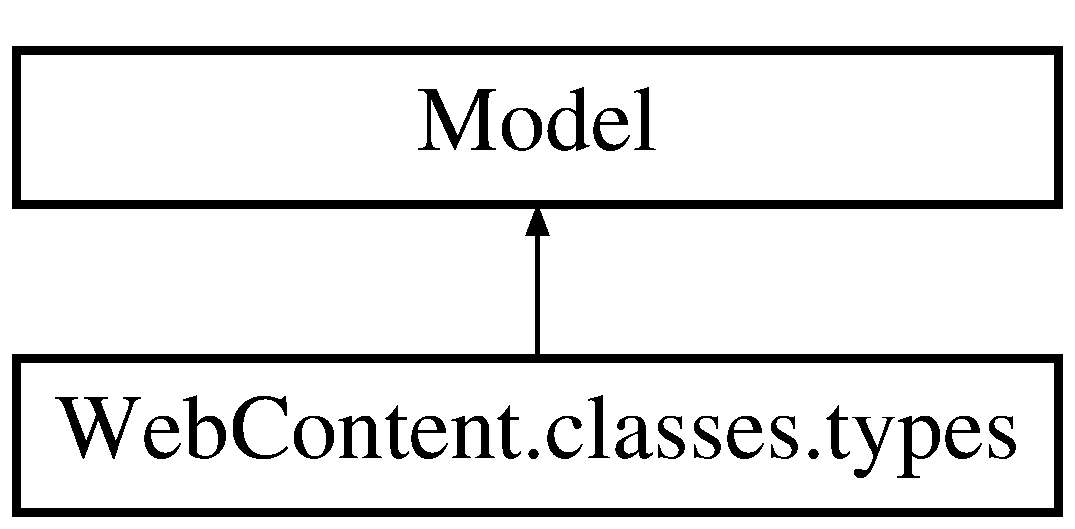
\includegraphics[height=2.000000cm]{class_web_content_1_1classes_1_1types}
\end{center}
\end{figure}
\subsection*{Public Member Functions}
\begin{DoxyCompactItemize}
\item 
def \hyperlink{class_web_content_1_1classes_1_1types_a87e09373df434b5bd47377d8399af113}{\+\_\+\+\_\+init\+\_\+\+\_\+} (self, \hyperlink{class_web_content_1_1classes_1_1types_a14ba7df18201fb701b0408d06bc4c058}{Type})
\item 
def \hyperlink{class_web_content_1_1classes_1_1types_ad63c238527b3bf635f67442625dc976e}{\+\_\+\+\_\+repr\+\_\+\+\_\+} (self)
\end{DoxyCompactItemize}
\subsection*{Static Public Attributes}
\begin{DoxyCompactItemize}
\item 
\hyperlink{class_web_content_1_1classes_1_1types_a14ba7df18201fb701b0408d06bc4c058}{Type} = db.\+Column(\textquotesingle{}Type\textquotesingle{}, db.\+String(45), primary\+\_\+key=True)
\end{DoxyCompactItemize}


\subsection{Constructor \& Destructor Documentation}
\mbox{\Hypertarget{class_web_content_1_1classes_1_1types_a87e09373df434b5bd47377d8399af113}\label{class_web_content_1_1classes_1_1types_a87e09373df434b5bd47377d8399af113}} 
\index{Web\+Content\+::classes\+::types@{Web\+Content\+::classes\+::types}!\+\_\+\+\_\+init\+\_\+\+\_\+@{\+\_\+\+\_\+init\+\_\+\+\_\+}}
\index{\+\_\+\+\_\+init\+\_\+\+\_\+@{\+\_\+\+\_\+init\+\_\+\+\_\+}!Web\+Content\+::classes\+::types@{Web\+Content\+::classes\+::types}}
\subsubsection{\texorpdfstring{\+\_\+\+\_\+init\+\_\+\+\_\+()}{\_\_init\_\_()}}
{\footnotesize\ttfamily def Web\+Content.\+classes.\+types.\+\_\+\+\_\+init\+\_\+\+\_\+ (\begin{DoxyParamCaption}\item[{}]{self,  }\item[{}]{Type }\end{DoxyParamCaption})}



\subsection{Member Function Documentation}
\mbox{\Hypertarget{class_web_content_1_1classes_1_1types_ad63c238527b3bf635f67442625dc976e}\label{class_web_content_1_1classes_1_1types_ad63c238527b3bf635f67442625dc976e}} 
\index{Web\+Content\+::classes\+::types@{Web\+Content\+::classes\+::types}!\+\_\+\+\_\+repr\+\_\+\+\_\+@{\+\_\+\+\_\+repr\+\_\+\+\_\+}}
\index{\+\_\+\+\_\+repr\+\_\+\+\_\+@{\+\_\+\+\_\+repr\+\_\+\+\_\+}!Web\+Content\+::classes\+::types@{Web\+Content\+::classes\+::types}}
\subsubsection{\texorpdfstring{\+\_\+\+\_\+repr\+\_\+\+\_\+()}{\_\_repr\_\_()}}
{\footnotesize\ttfamily def Web\+Content.\+classes.\+types.\+\_\+\+\_\+repr\+\_\+\+\_\+ (\begin{DoxyParamCaption}\item[{}]{self }\end{DoxyParamCaption})}



\subsection{Member Data Documentation}
\mbox{\Hypertarget{class_web_content_1_1classes_1_1types_a14ba7df18201fb701b0408d06bc4c058}\label{class_web_content_1_1classes_1_1types_a14ba7df18201fb701b0408d06bc4c058}} 
\index{Web\+Content\+::classes\+::types@{Web\+Content\+::classes\+::types}!Type@{Type}}
\index{Type@{Type}!Web\+Content\+::classes\+::types@{Web\+Content\+::classes\+::types}}
\subsubsection{\texorpdfstring{Type}{Type}}
{\footnotesize\ttfamily Web\+Content.\+classes.\+types.\+Type = db.\+Column(\textquotesingle{}Type\textquotesingle{}, db.\+String(45), primary\+\_\+key=True)\hspace{0.3cm}{\ttfamily [static]}}



The documentation for this class was generated from the following file\+:\begin{DoxyCompactItemize}
\item 
\hyperlink{classes_8py}{classes.\+py}\end{DoxyCompactItemize}

\hypertarget{class_web_content_1_1classes_1_1users}{}\section{Web\+Content.\+classes.\+users Class Reference}
\label{class_web_content_1_1classes_1_1users}\index{Web\+Content.\+classes.\+users@{Web\+Content.\+classes.\+users}}
Inheritance diagram for Web\+Content.\+classes.\+users\+:\begin{figure}[H]
\begin{center}
\leavevmode
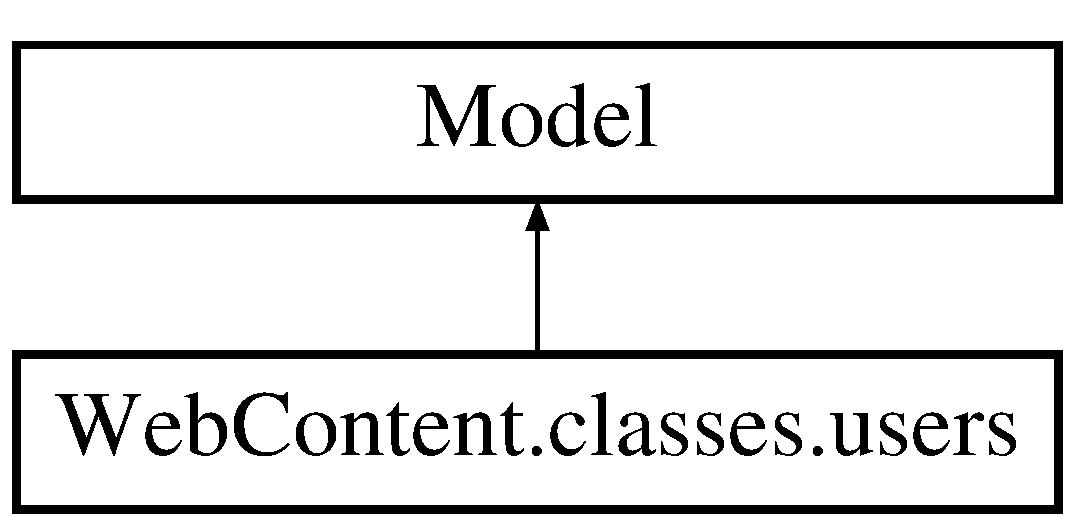
\includegraphics[height=2.000000cm]{class_web_content_1_1classes_1_1users}
\end{center}
\end{figure}
\subsection*{Public Member Functions}
\begin{DoxyCompactItemize}
\item 
def \hyperlink{class_web_content_1_1classes_1_1users_aa7a3c863509284695380f9e80022fbb7}{\+\_\+\+\_\+init\+\_\+\+\_\+} (self, \hyperlink{class_web_content_1_1classes_1_1users_ac626a21b539eab7dfd3170533ff98fad}{id\+Users}, \hyperlink{class_web_content_1_1classes_1_1users_a083d6c2ba8164a0edfdfba1e889829a4}{User}, \hyperlink{class_web_content_1_1classes_1_1users_a5e0e733ebeee5a02bcf563995196f295}{Password}, \hyperlink{class_web_content_1_1classes_1_1users_a0cff7737b58d91bf3502af5813c811d2}{Department}, \hyperlink{class_web_content_1_1classes_1_1users_aa3bdfac54124d297b6ac81a2ba5564f7}{Email})
\item 
def \hyperlink{class_web_content_1_1classes_1_1users_a84e8d242e4e64e56b9a038f2927ae71b}{\+\_\+\+\_\+repr\+\_\+\+\_\+} (self)
\end{DoxyCompactItemize}
\subsection*{Static Public Attributes}
\begin{DoxyCompactItemize}
\item 
\hyperlink{class_web_content_1_1classes_1_1users_ac626a21b539eab7dfd3170533ff98fad}{id\+Users} = db.\+Column(\textquotesingle{}id\+Users\textquotesingle{}, db.\+Integer, primary\+\_\+key=True)
\item 
\hyperlink{class_web_content_1_1classes_1_1users_a083d6c2ba8164a0edfdfba1e889829a4}{User} = db.\+Column(\textquotesingle{}User\textquotesingle{}, db.\+String(45))
\item 
\hyperlink{class_web_content_1_1classes_1_1users_a5e0e733ebeee5a02bcf563995196f295}{Password} = db.\+Column(\textquotesingle{}Password\textquotesingle{}, db.\+String(45))
\item 
\hyperlink{class_web_content_1_1classes_1_1users_a0cff7737b58d91bf3502af5813c811d2}{Department} = db.\+Column(\textquotesingle{}Department\textquotesingle{}, db.\+String(45))
\item 
\hyperlink{class_web_content_1_1classes_1_1users_aa3bdfac54124d297b6ac81a2ba5564f7}{Email} = db.\+Column(\textquotesingle{}Email\textquotesingle{}, db.\+String(45))
\end{DoxyCompactItemize}


\subsection{Constructor \& Destructor Documentation}
\mbox{\Hypertarget{class_web_content_1_1classes_1_1users_aa7a3c863509284695380f9e80022fbb7}\label{class_web_content_1_1classes_1_1users_aa7a3c863509284695380f9e80022fbb7}} 
\index{Web\+Content\+::classes\+::users@{Web\+Content\+::classes\+::users}!\+\_\+\+\_\+init\+\_\+\+\_\+@{\+\_\+\+\_\+init\+\_\+\+\_\+}}
\index{\+\_\+\+\_\+init\+\_\+\+\_\+@{\+\_\+\+\_\+init\+\_\+\+\_\+}!Web\+Content\+::classes\+::users@{Web\+Content\+::classes\+::users}}
\subsubsection{\texorpdfstring{\+\_\+\+\_\+init\+\_\+\+\_\+()}{\_\_init\_\_()}}
{\footnotesize\ttfamily def Web\+Content.\+classes.\+users.\+\_\+\+\_\+init\+\_\+\+\_\+ (\begin{DoxyParamCaption}\item[{}]{self,  }\item[{}]{id\+Users,  }\item[{}]{User,  }\item[{}]{Password,  }\item[{}]{Department,  }\item[{}]{Email }\end{DoxyParamCaption})}



\subsection{Member Function Documentation}
\mbox{\Hypertarget{class_web_content_1_1classes_1_1users_a84e8d242e4e64e56b9a038f2927ae71b}\label{class_web_content_1_1classes_1_1users_a84e8d242e4e64e56b9a038f2927ae71b}} 
\index{Web\+Content\+::classes\+::users@{Web\+Content\+::classes\+::users}!\+\_\+\+\_\+repr\+\_\+\+\_\+@{\+\_\+\+\_\+repr\+\_\+\+\_\+}}
\index{\+\_\+\+\_\+repr\+\_\+\+\_\+@{\+\_\+\+\_\+repr\+\_\+\+\_\+}!Web\+Content\+::classes\+::users@{Web\+Content\+::classes\+::users}}
\subsubsection{\texorpdfstring{\+\_\+\+\_\+repr\+\_\+\+\_\+()}{\_\_repr\_\_()}}
{\footnotesize\ttfamily def Web\+Content.\+classes.\+users.\+\_\+\+\_\+repr\+\_\+\+\_\+ (\begin{DoxyParamCaption}\item[{}]{self }\end{DoxyParamCaption})}



\subsection{Member Data Documentation}
\mbox{\Hypertarget{class_web_content_1_1classes_1_1users_a0cff7737b58d91bf3502af5813c811d2}\label{class_web_content_1_1classes_1_1users_a0cff7737b58d91bf3502af5813c811d2}} 
\index{Web\+Content\+::classes\+::users@{Web\+Content\+::classes\+::users}!Department@{Department}}
\index{Department@{Department}!Web\+Content\+::classes\+::users@{Web\+Content\+::classes\+::users}}
\subsubsection{\texorpdfstring{Department}{Department}}
{\footnotesize\ttfamily Web\+Content.\+classes.\+users.\+Department = db.\+Column(\textquotesingle{}Department\textquotesingle{}, db.\+String(45))\hspace{0.3cm}{\ttfamily [static]}}

\mbox{\Hypertarget{class_web_content_1_1classes_1_1users_aa3bdfac54124d297b6ac81a2ba5564f7}\label{class_web_content_1_1classes_1_1users_aa3bdfac54124d297b6ac81a2ba5564f7}} 
\index{Web\+Content\+::classes\+::users@{Web\+Content\+::classes\+::users}!Email@{Email}}
\index{Email@{Email}!Web\+Content\+::classes\+::users@{Web\+Content\+::classes\+::users}}
\subsubsection{\texorpdfstring{Email}{Email}}
{\footnotesize\ttfamily Web\+Content.\+classes.\+users.\+Email = db.\+Column(\textquotesingle{}Email\textquotesingle{}, db.\+String(45))\hspace{0.3cm}{\ttfamily [static]}}

\mbox{\Hypertarget{class_web_content_1_1classes_1_1users_ac626a21b539eab7dfd3170533ff98fad}\label{class_web_content_1_1classes_1_1users_ac626a21b539eab7dfd3170533ff98fad}} 
\index{Web\+Content\+::classes\+::users@{Web\+Content\+::classes\+::users}!id\+Users@{id\+Users}}
\index{id\+Users@{id\+Users}!Web\+Content\+::classes\+::users@{Web\+Content\+::classes\+::users}}
\subsubsection{\texorpdfstring{id\+Users}{idUsers}}
{\footnotesize\ttfamily Web\+Content.\+classes.\+users.\+id\+Users = db.\+Column(\textquotesingle{}id\+Users\textquotesingle{}, db.\+Integer, primary\+\_\+key=True)\hspace{0.3cm}{\ttfamily [static]}}

\mbox{\Hypertarget{class_web_content_1_1classes_1_1users_a5e0e733ebeee5a02bcf563995196f295}\label{class_web_content_1_1classes_1_1users_a5e0e733ebeee5a02bcf563995196f295}} 
\index{Web\+Content\+::classes\+::users@{Web\+Content\+::classes\+::users}!Password@{Password}}
\index{Password@{Password}!Web\+Content\+::classes\+::users@{Web\+Content\+::classes\+::users}}
\subsubsection{\texorpdfstring{Password}{Password}}
{\footnotesize\ttfamily Web\+Content.\+classes.\+users.\+Password = db.\+Column(\textquotesingle{}Password\textquotesingle{}, db.\+String(45))\hspace{0.3cm}{\ttfamily [static]}}

\mbox{\Hypertarget{class_web_content_1_1classes_1_1users_a083d6c2ba8164a0edfdfba1e889829a4}\label{class_web_content_1_1classes_1_1users_a083d6c2ba8164a0edfdfba1e889829a4}} 
\index{Web\+Content\+::classes\+::users@{Web\+Content\+::classes\+::users}!User@{User}}
\index{User@{User}!Web\+Content\+::classes\+::users@{Web\+Content\+::classes\+::users}}
\subsubsection{\texorpdfstring{User}{User}}
{\footnotesize\ttfamily Web\+Content.\+classes.\+users.\+User = db.\+Column(\textquotesingle{}User\textquotesingle{}, db.\+String(45))\hspace{0.3cm}{\ttfamily [static]}}



The documentation for this class was generated from the following file\+:\begin{DoxyCompactItemize}
\item 
\hyperlink{classes_8py}{classes.\+py}\end{DoxyCompactItemize}

\hypertarget{class_web_content_1_1classes_1_1venues}{}\section{Web\+Content.\+classes.\+venues Class Reference}
\label{class_web_content_1_1classes_1_1venues}\index{Web\+Content.\+classes.\+venues@{Web\+Content.\+classes.\+venues}}
Inheritance diagram for Web\+Content.\+classes.\+venues\+:\begin{figure}[H]
\begin{center}
\leavevmode
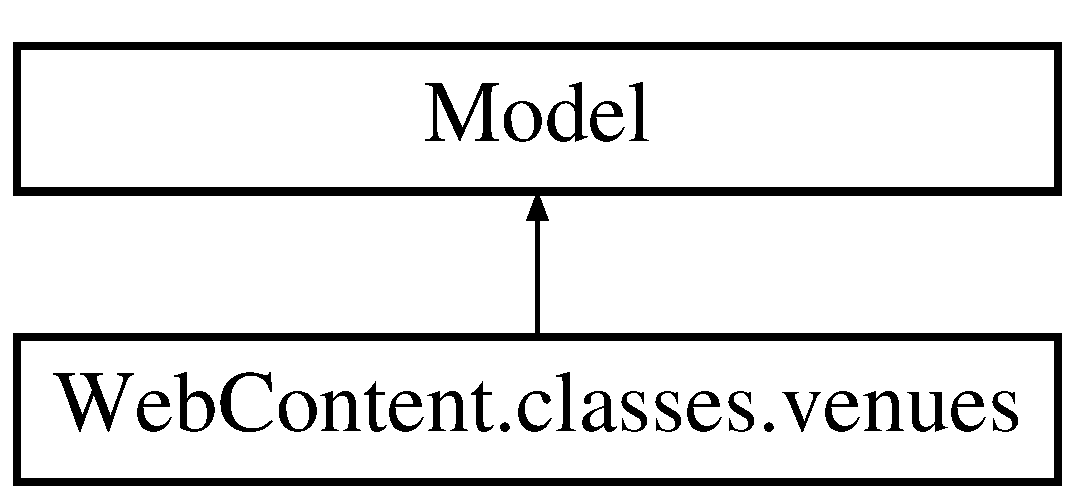
\includegraphics[height=2.000000cm]{class_web_content_1_1classes_1_1venues}
\end{center}
\end{figure}
\subsection*{Public Member Functions}
\begin{DoxyCompactItemize}
\item 
def \hyperlink{class_web_content_1_1classes_1_1venues_ad7ff0f4c4610450e6d2afb55ebab01cb}{\+\_\+\+\_\+init\+\_\+\+\_\+} (self, \hyperlink{class_web_content_1_1classes_1_1venues_a9b9a18b684f7b9e71a8068443cd008d2}{venue\+Name}, \hyperlink{class_web_content_1_1classes_1_1venues_a5e482b9cf50927587cd0940be0a65eb4}{Address}, \hyperlink{class_web_content_1_1classes_1_1venues_a1575dda3b6e4b1ba7b89b03e31cfb0c9}{City}, \hyperlink{class_web_content_1_1classes_1_1venues_ac3846ed9b5b20948852b9374dd35fd22}{Zip}, \hyperlink{class_web_content_1_1classes_1_1venues_a5bf3b821cbc920a6f970c36577a451a4}{Phone}, \hyperlink{class_web_content_1_1classes_1_1venues_a2bcc906a39635f4e154cff0a5d1070ad}{contact\+Name}, \hyperlink{class_web_content_1_1classes_1_1venues_a68472a0e51533d6ee114f3668e262bd6}{layout}, \hyperlink{class_web_content_1_1classes_1_1venues_a4c87fdcce94a8d92e888b0ef112da682}{U\+RL})
\item 
def \hyperlink{class_web_content_1_1classes_1_1venues_a1c806e25e7eb1c18ba58a51817120f00}{\+\_\+\+\_\+repr\+\_\+\+\_\+} (self)
\end{DoxyCompactItemize}
\subsection*{Static Public Attributes}
\begin{DoxyCompactItemize}
\item 
\hyperlink{class_web_content_1_1classes_1_1venues_a9b9a18b684f7b9e71a8068443cd008d2}{venue\+Name} = db.\+Column(\textquotesingle{}venue\+Name\textquotesingle{}, db.\+String(55), primary\+\_\+key=True)
\item 
\hyperlink{class_web_content_1_1classes_1_1venues_a5e482b9cf50927587cd0940be0a65eb4}{Address} = db.\+Column(\textquotesingle{}Address\textquotesingle{}, db.\+String(255))
\item 
\hyperlink{class_web_content_1_1classes_1_1venues_a1575dda3b6e4b1ba7b89b03e31cfb0c9}{City} = db.\+Column(\textquotesingle{}City\textquotesingle{}, db.\+String(255))
\item 
\hyperlink{class_web_content_1_1classes_1_1venues_ac3846ed9b5b20948852b9374dd35fd22}{Zip} = db.\+Column(\textquotesingle{}Zip\textquotesingle{}, db.\+String(255))
\item 
\hyperlink{class_web_content_1_1classes_1_1venues_a5bf3b821cbc920a6f970c36577a451a4}{Phone} = db.\+Column(\textquotesingle{}Phone\textquotesingle{}, db.\+String(14))
\item 
\hyperlink{class_web_content_1_1classes_1_1venues_a2bcc906a39635f4e154cff0a5d1070ad}{contact\+Name} = db.\+Column(\textquotesingle{}contact\+Name\textquotesingle{}, db.\+String(55))
\item 
\hyperlink{class_web_content_1_1classes_1_1venues_a68472a0e51533d6ee114f3668e262bd6}{layout} = db.\+Column(\textquotesingle{}layout\textquotesingle{}, db.\+String(255))
\item 
\hyperlink{class_web_content_1_1classes_1_1venues_a4c87fdcce94a8d92e888b0ef112da682}{U\+RL} = db.\+Column(\textquotesingle{}U\+RL\textquotesingle{}, db.\+String(55))
\end{DoxyCompactItemize}


\subsection{Constructor \& Destructor Documentation}
\mbox{\Hypertarget{class_web_content_1_1classes_1_1venues_ad7ff0f4c4610450e6d2afb55ebab01cb}\label{class_web_content_1_1classes_1_1venues_ad7ff0f4c4610450e6d2afb55ebab01cb}} 
\index{Web\+Content\+::classes\+::venues@{Web\+Content\+::classes\+::venues}!\+\_\+\+\_\+init\+\_\+\+\_\+@{\+\_\+\+\_\+init\+\_\+\+\_\+}}
\index{\+\_\+\+\_\+init\+\_\+\+\_\+@{\+\_\+\+\_\+init\+\_\+\+\_\+}!Web\+Content\+::classes\+::venues@{Web\+Content\+::classes\+::venues}}
\subsubsection{\texorpdfstring{\+\_\+\+\_\+init\+\_\+\+\_\+()}{\_\_init\_\_()}}
{\footnotesize\ttfamily def Web\+Content.\+classes.\+venues.\+\_\+\+\_\+init\+\_\+\+\_\+ (\begin{DoxyParamCaption}\item[{}]{self,  }\item[{}]{venue\+Name,  }\item[{}]{Address,  }\item[{}]{City,  }\item[{}]{Zip,  }\item[{}]{Phone,  }\item[{}]{contact\+Name,  }\item[{}]{layout,  }\item[{}]{U\+RL }\end{DoxyParamCaption})}



\subsection{Member Function Documentation}
\mbox{\Hypertarget{class_web_content_1_1classes_1_1venues_a1c806e25e7eb1c18ba58a51817120f00}\label{class_web_content_1_1classes_1_1venues_a1c806e25e7eb1c18ba58a51817120f00}} 
\index{Web\+Content\+::classes\+::venues@{Web\+Content\+::classes\+::venues}!\+\_\+\+\_\+repr\+\_\+\+\_\+@{\+\_\+\+\_\+repr\+\_\+\+\_\+}}
\index{\+\_\+\+\_\+repr\+\_\+\+\_\+@{\+\_\+\+\_\+repr\+\_\+\+\_\+}!Web\+Content\+::classes\+::venues@{Web\+Content\+::classes\+::venues}}
\subsubsection{\texorpdfstring{\+\_\+\+\_\+repr\+\_\+\+\_\+()}{\_\_repr\_\_()}}
{\footnotesize\ttfamily def Web\+Content.\+classes.\+venues.\+\_\+\+\_\+repr\+\_\+\+\_\+ (\begin{DoxyParamCaption}\item[{}]{self }\end{DoxyParamCaption})}



\subsection{Member Data Documentation}
\mbox{\Hypertarget{class_web_content_1_1classes_1_1venues_a5e482b9cf50927587cd0940be0a65eb4}\label{class_web_content_1_1classes_1_1venues_a5e482b9cf50927587cd0940be0a65eb4}} 
\index{Web\+Content\+::classes\+::venues@{Web\+Content\+::classes\+::venues}!Address@{Address}}
\index{Address@{Address}!Web\+Content\+::classes\+::venues@{Web\+Content\+::classes\+::venues}}
\subsubsection{\texorpdfstring{Address}{Address}}
{\footnotesize\ttfamily Web\+Content.\+classes.\+venues.\+Address = db.\+Column(\textquotesingle{}Address\textquotesingle{}, db.\+String(255))\hspace{0.3cm}{\ttfamily [static]}}

\mbox{\Hypertarget{class_web_content_1_1classes_1_1venues_a1575dda3b6e4b1ba7b89b03e31cfb0c9}\label{class_web_content_1_1classes_1_1venues_a1575dda3b6e4b1ba7b89b03e31cfb0c9}} 
\index{Web\+Content\+::classes\+::venues@{Web\+Content\+::classes\+::venues}!City@{City}}
\index{City@{City}!Web\+Content\+::classes\+::venues@{Web\+Content\+::classes\+::venues}}
\subsubsection{\texorpdfstring{City}{City}}
{\footnotesize\ttfamily Web\+Content.\+classes.\+venues.\+City = db.\+Column(\textquotesingle{}City\textquotesingle{}, db.\+String(255))\hspace{0.3cm}{\ttfamily [static]}}

\mbox{\Hypertarget{class_web_content_1_1classes_1_1venues_a2bcc906a39635f4e154cff0a5d1070ad}\label{class_web_content_1_1classes_1_1venues_a2bcc906a39635f4e154cff0a5d1070ad}} 
\index{Web\+Content\+::classes\+::venues@{Web\+Content\+::classes\+::venues}!contact\+Name@{contact\+Name}}
\index{contact\+Name@{contact\+Name}!Web\+Content\+::classes\+::venues@{Web\+Content\+::classes\+::venues}}
\subsubsection{\texorpdfstring{contact\+Name}{contactName}}
{\footnotesize\ttfamily Web\+Content.\+classes.\+venues.\+contact\+Name = db.\+Column(\textquotesingle{}contact\+Name\textquotesingle{}, db.\+String(55))\hspace{0.3cm}{\ttfamily [static]}}

\mbox{\Hypertarget{class_web_content_1_1classes_1_1venues_a68472a0e51533d6ee114f3668e262bd6}\label{class_web_content_1_1classes_1_1venues_a68472a0e51533d6ee114f3668e262bd6}} 
\index{Web\+Content\+::classes\+::venues@{Web\+Content\+::classes\+::venues}!layout@{layout}}
\index{layout@{layout}!Web\+Content\+::classes\+::venues@{Web\+Content\+::classes\+::venues}}
\subsubsection{\texorpdfstring{layout}{layout}}
{\footnotesize\ttfamily Web\+Content.\+classes.\+venues.\+layout = db.\+Column(\textquotesingle{}layout\textquotesingle{}, db.\+String(255))\hspace{0.3cm}{\ttfamily [static]}}

\mbox{\Hypertarget{class_web_content_1_1classes_1_1venues_a5bf3b821cbc920a6f970c36577a451a4}\label{class_web_content_1_1classes_1_1venues_a5bf3b821cbc920a6f970c36577a451a4}} 
\index{Web\+Content\+::classes\+::venues@{Web\+Content\+::classes\+::venues}!Phone@{Phone}}
\index{Phone@{Phone}!Web\+Content\+::classes\+::venues@{Web\+Content\+::classes\+::venues}}
\subsubsection{\texorpdfstring{Phone}{Phone}}
{\footnotesize\ttfamily Web\+Content.\+classes.\+venues.\+Phone = db.\+Column(\textquotesingle{}Phone\textquotesingle{}, db.\+String(14))\hspace{0.3cm}{\ttfamily [static]}}

\mbox{\Hypertarget{class_web_content_1_1classes_1_1venues_a4c87fdcce94a8d92e888b0ef112da682}\label{class_web_content_1_1classes_1_1venues_a4c87fdcce94a8d92e888b0ef112da682}} 
\index{Web\+Content\+::classes\+::venues@{Web\+Content\+::classes\+::venues}!U\+RL@{U\+RL}}
\index{U\+RL@{U\+RL}!Web\+Content\+::classes\+::venues@{Web\+Content\+::classes\+::venues}}
\subsubsection{\texorpdfstring{U\+RL}{URL}}
{\footnotesize\ttfamily Web\+Content.\+classes.\+venues.\+U\+RL = db.\+Column(\textquotesingle{}U\+RL\textquotesingle{}, db.\+String(55))\hspace{0.3cm}{\ttfamily [static]}}

\mbox{\Hypertarget{class_web_content_1_1classes_1_1venues_a9b9a18b684f7b9e71a8068443cd008d2}\label{class_web_content_1_1classes_1_1venues_a9b9a18b684f7b9e71a8068443cd008d2}} 
\index{Web\+Content\+::classes\+::venues@{Web\+Content\+::classes\+::venues}!venue\+Name@{venue\+Name}}
\index{venue\+Name@{venue\+Name}!Web\+Content\+::classes\+::venues@{Web\+Content\+::classes\+::venues}}
\subsubsection{\texorpdfstring{venue\+Name}{venueName}}
{\footnotesize\ttfamily Web\+Content.\+classes.\+venues.\+venue\+Name = db.\+Column(\textquotesingle{}venue\+Name\textquotesingle{}, db.\+String(55), primary\+\_\+key=True)\hspace{0.3cm}{\ttfamily [static]}}

\mbox{\Hypertarget{class_web_content_1_1classes_1_1venues_ac3846ed9b5b20948852b9374dd35fd22}\label{class_web_content_1_1classes_1_1venues_ac3846ed9b5b20948852b9374dd35fd22}} 
\index{Web\+Content\+::classes\+::venues@{Web\+Content\+::classes\+::venues}!Zip@{Zip}}
\index{Zip@{Zip}!Web\+Content\+::classes\+::venues@{Web\+Content\+::classes\+::venues}}
\subsubsection{\texorpdfstring{Zip}{Zip}}
{\footnotesize\ttfamily Web\+Content.\+classes.\+venues.\+Zip = db.\+Column(\textquotesingle{}Zip\textquotesingle{}, db.\+String(255))\hspace{0.3cm}{\ttfamily [static]}}



The documentation for this class was generated from the following file\+:\begin{DoxyCompactItemize}
\item 
\hyperlink{classes_8py}{classes.\+py}\end{DoxyCompactItemize}

\chapter{File Documentation}
\hypertarget{____init_____8py}{}\section{C\+:/\+Users/\+Antonio/\+Documents/\+Git\+Hub/\+Spitfire\+Capstone/\+Web\+Content/\+\_\+\+\_\+init\+\_\+\+\_\+.py File Reference}
\label{____init_____8py}\index{C\+:/\+Users/\+Antonio/\+Documents/\+Git\+Hub/\+Spitfire\+Capstone/\+Web\+Content/\+\_\+\+\_\+init\+\_\+\+\_\+.\+py@{C\+:/\+Users/\+Antonio/\+Documents/\+Git\+Hub/\+Spitfire\+Capstone/\+Web\+Content/\+\_\+\+\_\+init\+\_\+\+\_\+.\+py}}
\subsection*{Namespaces}
\begin{DoxyCompactItemize}
\item 
 \hyperlink{namespace_web_content}{Web\+Content}
\end{DoxyCompactItemize}

\hypertarget{app_8py}{}\section{C\+:/\+Users/\+Antonio/\+Documents/\+Git\+Hub/\+Spitfire\+Capstone/\+Web\+Content/app.py File Reference}
\label{app_8py}\index{C\+:/\+Users/\+Antonio/\+Documents/\+Git\+Hub/\+Spitfire\+Capstone/\+Web\+Content/app.\+py@{C\+:/\+Users/\+Antonio/\+Documents/\+Git\+Hub/\+Spitfire\+Capstone/\+Web\+Content/app.\+py}}
\subsection*{Namespaces}
\begin{DoxyCompactItemize}
\item 
 \hyperlink{namespace_web_content_1_1app}{Web\+Content.\+app}
\end{DoxyCompactItemize}
\subsection*{Functions}
\begin{DoxyCompactItemize}
\item 
def \hyperlink{namespace_web_content_1_1app_ab0090e2c92ec892cf11fed49d580737a}{Web\+Content.\+app.\+home} ()
\item 
def \hyperlink{namespace_web_content_1_1app_ac220a4f6d552ae239a9fe5a933eb4c0d}{Web\+Content.\+app.\+welcome} ()
\item 
def \hyperlink{namespace_web_content_1_1app_a1e55cf68c2c2c883c82749a8725e068c}{Web\+Content.\+app.\+login} ()
\item 
def \hyperlink{namespace_web_content_1_1app_aeb0d3df489a674be05033bd0ba98e7a6}{Web\+Content.\+app.\+database} ()
\item 
def \hyperlink{namespace_web_content_1_1app_a01e890f5f74756a5e0db012e87a3bb32}{Web\+Content.\+app.\+add} ()
\item 
def \hyperlink{namespace_web_content_1_1app_a2f6071690c83608f94abb72589ab7527}{Web\+Content.\+app.\+update} (id\+Items)
\item 
def \hyperlink{namespace_web_content_1_1app_a280b9c530dfd4125df19a186218bb132}{Web\+Content.\+app.\+delete} (id\+Items)
\item 
def \hyperlink{namespace_web_content_1_1app_a368b9d1da5b4c987484797ecce9aabc9}{Web\+Content.\+app.\+calendar} ()
\item 
def \hyperlink{namespace_web_content_1_1app_a6d7ee2ff030bada6042b07189d92a01c}{Web\+Content.\+app.\+search} ()
\item 
def \hyperlink{namespace_web_content_1_1app_a26131900d865fe102463bc8eb3a797ef}{Web\+Content.\+app.\+search\+Show} ()
\item 
def \hyperlink{namespace_web_content_1_1app_afe68584aa29f9b47108d88d14650c05f}{Web\+Content.\+app.\+account} ()
\item 
def \hyperlink{namespace_web_content_1_1app_ada0f5f23829cfced6b4d13fbf597f82b}{Web\+Content.\+app.\+add\+Show} ()
\item 
def \hyperlink{namespace_web_content_1_1app_a6e8308958b72dbb2468ed92b6389d990}{Web\+Content.\+app.\+gear\+List} ()
\item 
def \hyperlink{namespace_web_content_1_1app_a1aefd89635932b2165c829b462687b74}{Web\+Content.\+app.\+gear\+List\+Welcome} ()
\item 
def \hyperlink{namespace_web_content_1_1app_a6be53570f8642dc8f71ad686863336cc}{Web\+Content.\+app.\+show} (id\+Shows)
\item 
def \hyperlink{namespace_web_content_1_1app_a8a745fdd281519fdc01c26e4ebbc5f87}{Web\+Content.\+app.\+show\+Gear} (id\+Shows)
\item 
def \hyperlink{namespace_web_content_1_1app_a9e50daef82abeaa1acba1829fcd2b9ae}{Web\+Content.\+app.\+daily\+Task} ()
\item 
def \hyperlink{namespace_web_content_1_1app_a74ab25eca92d4f0315c1920a1101f366}{Web\+Content.\+app.\+add\+Daily\+Task} ()
\item 
def \hyperlink{namespace_web_content_1_1app_af2ca8754b886a2732a45b71b8a53f185}{Web\+Content.\+app.\+delete\+Task} (iddaily\+\_\+task)
\item 
def \hyperlink{namespace_web_content_1_1app_ad3f479298a258fcecb0cf0fae0c3e6de}{Web\+Content.\+app.\+gantt\+View} ()
\item 
def \hyperlink{namespace_web_content_1_1app_a243cda6941738022b0168abcbe9d8e7d}{Web\+Content.\+app.\+contacts} ()
\item 
def \hyperlink{namespace_web_content_1_1app_a32b908258de025be7473e15954f4683c}{Web\+Content.\+app.\+add\+Contact} ()
\item 
def \hyperlink{namespace_web_content_1_1app_a8934b836311d8645b794937a4665b687}{Web\+Content.\+app.\+delete\+Contact} (contact\+Name)
\item 
def \hyperlink{namespace_web_content_1_1app_a6192c461f4e0e0a2310f43f91f2724ad}{Web\+Content.\+app.\+update\+Contact} (contact\+Name)
\item 
def \hyperlink{namespace_web_content_1_1app_a73068e2cc15ecd211e7fbdbe744dbcf0}{Web\+Content.\+app.\+item\+List} ()
\item 
def \hyperlink{namespace_web_content_1_1app_a52178c26cbe8ed1b16427622b4dc1165}{Web\+Content.\+app.\+add\+Gear} (id\+Shows, id\+Items)
\item 
def \hyperlink{namespace_web_content_1_1app_a7223fddf3b4dbcc57318bd9b85b30c5d}{Web\+Content.\+app.\+return\+Item} (id\+Shows, idallocation\+\_\+table)
\end{DoxyCompactItemize}
\subsection*{Variables}
\begin{DoxyCompactItemize}
\item 
\hyperlink{namespace_web_content_1_1app_a52716e6e08bae668f90c903a1f4e2f10}{Web\+Content.\+app.\+app} = Flask(\+\_\+\+\_\+name\+\_\+\+\_\+)
\item 
\hyperlink{namespace_web_content_1_1app_a317646b91bdcf24c176d3bfc065083f3}{Web\+Content.\+app.\+db} = S\+Q\+L\+Alchemy(app)
\item 
\hyperlink{namespace_web_content_1_1app_a6092358451315e755637b56d42326052}{Web\+Content.\+app.\+secret\+\_\+key}
\item 
list \hyperlink{namespace_web_content_1_1app_a8a9f65f156a7f89775a11e01516c5400}{Web\+Content.\+app.\+Id\+List} = \mbox{[}$\,$\mbox{]}
\item 
\hyperlink{namespace_web_content_1_1app_ac91170bea34c6458f4262824618a18a2}{Web\+Content.\+app.\+debug}
\end{DoxyCompactItemize}

\hypertarget{classes_8py}{}\section{classes.\+py File Reference}
\label{classes_8py}\index{classes.\+py@{classes.\+py}}
\subsection*{Classes}
\begin{DoxyCompactItemize}
\item 
class \hyperlink{class_web_content_1_1classes_1_1users}{Web\+Content.\+classes.\+users}
\item 
class \hyperlink{class_web_content_1_1classes_1_1items}{Web\+Content.\+classes.\+items}
\item 
class \hyperlink{class_web_content_1_1classes_1_1_shows}{Web\+Content.\+classes.\+Shows}
\item 
class \hyperlink{class_web_content_1_1classes_1_1contacts}{Web\+Content.\+classes.\+contacts}
\item 
class \hyperlink{class_web_content_1_1classes_1_1job_gear}{Web\+Content.\+classes.\+job\+Gear}
\item 
class \hyperlink{class_web_content_1_1classes_1_1types}{Web\+Content.\+classes.\+types}
\item 
class \hyperlink{class_web_content_1_1classes_1_1venues}{Web\+Content.\+classes.\+venues}
\end{DoxyCompactItemize}
\subsection*{Namespaces}
\begin{DoxyCompactItemize}
\item 
 \hyperlink{namespace_web_content_1_1classes}{Web\+Content.\+classes}
\end{DoxyCompactItemize}

%--- End generated contents ---

% Index
\backmatter
\newpage
\phantomsection
\clearemptydoublepage
\addcontentsline{toc}{chapter}{Index}
\printindex

\end{document}
